\documentclass[pdflatex,sn-mathphys-num]{sn-jnl}

%% ================================================================
%% Springer Nature Journal Article Template (sn-jnl Version 3.1)
%% Plant Disease Screening System — Research Paper
%% ================================================================

\usepackage{graphicx}%
\usepackage{multirow}%
\usepackage{amsmath,amssymb,amsfonts}%
\usepackage{amsthm}%
\usepackage[title]{appendix}%
\usepackage{xcolor}%
\usepackage{textcomp}%
\usepackage{booktabs}%
\usepackage{algorithm}%
\usepackage{algorithmicx}%
\usepackage{algpseudocode}%


\theoremstyle{thmstyleone}%
\newtheorem{theorem}{Theorem}%
\newtheorem{proposition}[theorem]{Proposition}%

\theoremstyle{thmstyletwo}%
\newtheorem{example}{Example}%
\newtheorem{remark}{Remark}%

\theoremstyle{thmstylethree}%
\newtheorem{definition}{Definition}%

\raggedbottom

%% ================================================================


\begin{document}

\title[Plant Disease Screening System]{Plant Disease Screening System with MobileNetV3-Small:
Implementation, Exploratory Results, and Validation Gaps}

\author*[1]{\fnm{Mohit} \sur{Sharma}}\email{mohit.12324849@lpu.in}
\author[1]{\fnm{Aniket} \sur{Kumar}}\equalcont{These authors contributed equally to this work.}\email{aniket.12325552@lpu.in}
\author[1]{\fnm{Raghav} \sur{Kumar}}\equalcont{These authors contributed equally to this work.}\email{raghavmumar23@lpu.in}

\affil*[1]{\orgdiv{Department of Computer Science and Engineering},
  \orgname{Lovely Professional University},
  \orgaddress{\city{Phagwara}, \state{Punjab}, \postcode{144411}, \country{India}}}

\abstract{
Plant diseases cause between 20\% and 40\% of global crop yield losses annually, imposing
severe threats to food security in developing economies where smallholder farmers lack
access to timely diagnostic expertise \citep{savary2019burden}. This paper presents a
comprehensive implementation and empirical evaluation of a CPU-deployable plant disease
screening system built upon a family of lightweight convolutional neural network
architectures trained on a combined PlantVillage and PlantDoc dataset comprising 56{,}433 images across 38 disease classes (40{,}151 training, 5{,}436 validation, 5{,}429 calibration, and 5{,}417 holdout test images, constructed after excluding 31 duplicate and conflicting records from the 54{,}305 PlantVillage source images). Four architectures are systematically benchmarked:
MobileNetV3-Small, MobileNetV3-Large, EfficientNet-B0, and ResNet18. All models are
trained with duplicate-aware data partitioning, cryptographically verified checkpoints,
and post-hoc temperature scaling calibration. On the reserved PlantVillage holdout test
partition (5{,}417 images), MobileNetV3-Large achieves the highest accuracy of 95.96\%
with a Macro-F1 of 94.52\%, while MobileNetV3-Small provides the best computational
efficiency at 9.42\,ms per single inference and 6.06\,MB disk footprint. External
evaluation on 236 natural-background PlantDoc images reveals a substantial domain shift
of approximately 56 percentage points, with the best-performing architecture reaching
only 41.53\% top-1 accuracy in unconstrained field conditions. A candidate-region
multi-scale sliding-window screening pipeline is proposed and evaluated against PlantDoc
bounding-box annotations, achieving 38.05\% leaf localization recall at IoU~$\geq~0.25$
after optimization---more than double the baseline recall of 18.14\%. Critical
limitations regarding domain generalization, clinical reliability, and application
integration are discussed transparently. The findings establish a reproducible baseline
for future work in field-deployable plant disease AI.
}

\keywords{Plant disease detection, Deep learning, MobileNetV3, Domain generalization, Candidate-region screening, Temperature calibration}

\maketitle

%% ================================================================
%% 1. INTRODUCTION
%% ================================================================

\section{Introduction}
\label{sec:introduction}

Agricultural crop losses attributable to fungal, bacterial, and viral plant diseases
represent one of the most pressing threats to global food security. \citet{savary2019burden}
estimated that pathogens and pests collectively reduce yields of the world's five major
staple crops---wheat, rice, maize, potato, and soybean---by 10\%–40\% annually. In many
low- and middle-income countries, smallholder farmers who cultivate the majority of food
are disproportionately impacted because they typically have limited access to plant
pathology expertise, agrochemical advisory services, or digital tools for timely disease
identification.

Computer vision and deep learning have emerged as promising technologies to democratise
plant disease diagnosis. The seminal work of \citet{mohanty2016} demonstrated that deep
convolutional neural networks (CNNs) could classify 26 diseases across 14 crop species
at over 99\% accuracy under controlled PlantVillage \citep{hughes2015plantvillage}
laboratory conditions. Subsequent work consistently replicated high in-domain accuracy
\citep{ferentinos2018deep,chen2020identification,atila2021plant}, fuelling optimism about
AI-driven agricultural diagnostics.

However, three critical gaps separate laboratory benchmarks from reliable field
deployment.

First, \textit{domain shift}: models trained exclusively on PlantVillage images---where
individual leaves are photographed against plain grey or black backgrounds---perform
substantially worse on natural photographs with complex backgrounds, variable lighting,
multi-leaf occlusion, and camera motion blur \citep{barbedo2016review,singh2020plant,dsouza2023generalization}.
\citet{toda2019deep} and \citet{thapa2020plant} confirmed that apparent accuracy improvements
on curated benchmarks frequently fail to transfer to in-field conditions.

Second, \textit{probability calibration}: modern CNNs are often overconfident or
underconfident in their predicted probabilities, limiting the utility of confidence
thresholds for clinical or autonomous decision-making \citep{guo2017calibration,minderer2021calibration}.
Without calibration, a model reporting 95\% confidence cannot be trusted to be correct
95\% of the time.

Third, \textit{whole-plant localization}: practical field photographs typically contain
multiple leaves, background vegetation, soil, and sky. Classifying the entire image as a
single class conflates contributions from healthy and diseased plant material
\citep{barbedo2018factors,ren2015fasterrcnn}.

This paper addresses all three gaps through a systematic, multi-phase experimental
programme. The contributions are:

\begin{enumerate}
  \item A reproducible dataset pipeline with duplicate-aware splitting, SHA-256 manifest
        verification, and strict partition isolation across training, validation,
        calibration, and holdout test sets.
  \item A comparative benchmark of four CNN architectures (MobileNetV3-Small,
        MobileNetV3-Large, EfficientNet-B0, ResNet18) trained and evaluated under
        identical experimental protocols on CPU hardware.
  \item Post-hoc temperature scaling calibration applied separately for each architecture
        using an isolated calibration partition, with pre- and post-calibration Expected
        Calibration Error (ECE) reported transparently.
  \item An independent external evaluation on 236 PlantDoc natural-background images,
        quantifying the domain gap without fine-tuning or threshold adaptation.
  \item A candidate-region screening pipeline using multi-scale sliding windows, Excess
        Green Index (ExG) foliar saliency filtering, 12\% context padding, and hybrid
        NMS, evaluated against 452 whole-leaf bounding-box annotations.
\end{enumerate}

\subsection{Research Gap}
\label{sec:research_gap}

A specific gap motivating this work was identified in prior exploratory research on the
same system: the initial MobileNetV3-Small checkpoint lacked verifiable training-split
provenance, the external PlantDoc evaluation had not been conducted, the calibrated
temperature parameter used offline differed from the application configuration, and no
multi-architecture comparison existed. This paper directly addresses each of these gaps
using completed experimental evidence from a structured five-phase research programme.

\subsection{Research Objectives}
\label{sec:objectives}

The primary objectives of this study are:
\begin{enumerate}[(i)]
  \item To establish a fully reproducible training protocol with cryptographic checkpoint
        provenance for all evaluated architectures.
  \item To quantify the classification performance of four lightweight CNN architectures
        on the controlled PlantVillage holdout test set.
  \item To evaluate cross-domain generalization on external, unconstrained PlantDoc images.
  \item To apply and evaluate post-hoc temperature scaling calibration for each architecture.
  \item To design, implement, and evaluate a multi-scale candidate-region screening
        pipeline for whole-plant field images.
  \item To identify and transparently document remaining performance gaps and
        architectural limitations.
\end{enumerate}

%% ================================================================
%% 2. LITERATURE REVIEW
%% ================================================================

\section{Literature Review}
\label{sec:literature_review}

\subsection{Deep Learning for Plant Disease Recognition}

The field of AI-based plant disease recognition has advanced rapidly since
\citet{mohanty2016} first demonstrated that CNNs trained on PlantVillage could
achieve near-human performance on a held-out test partition. Subsequent benchmarks
using AlexNet, VGG, Inception, and ResNet variants have consistently demonstrated
top-1 accuracies exceeding 95\% on PlantVillage's controlled imagery
\citep{ferentinos2018deep,too2019comparative}. \citet{kamilaris2018deep} provided
a comprehensive survey of deep learning applications across agricultural domains,
noting that image classification remains the most mature sub-task, while disease
localisation and severity estimation remain open challenges.

\subsection{CNN Architectures for Lightweight Deployment}

Resource-efficient CNN architectures are critical for deployment on mobile and
edge devices without GPU acceleration \citep{howard2017mobilenets}. The MobileNet
family introduced depthwise separable convolutions to reduce floating-point operations
per inference by approximately one order of magnitude relative to VGG-16
\citep{howard2017mobilenets}. MobileNetV3, proposed by \citet{howard2019mobilenetv3},
further integrated Neural Architecture Search (NAS), Squeeze-and-Excitation (SE)
attention modules \citep{hu2018squeeze}, and hard-swish activations to improve both
accuracy and latency on mobile hardware.

EfficientNet \citep{tan2019efficientnet} introduces compound scaling, a principled
method that simultaneously scales network depth, width, and resolution using a fixed
set of coefficients derived from NAS. EfficientNet-B0 serves as the smallest member
of this family and has been widely adopted in plant disease classification studies,
achieving strong accuracy with moderate parameter counts \citep{atila2021plant}.

ResNet \citep{he2016resnet} introduced skip connections that enable training of very
deep networks by enabling gradient flow through identity shortcuts. Despite being an
older architecture, ResNet-18 remains a competitive baseline due to its simplicity,
well-understood failure modes, and ease of transfer learning.

\subsection{PlantVillage and PlantDoc Benchmarks}

PlantVillage \citep{hughes2015plantvillage} provides 54{,}305 images across 38 plant
disease and health classes, all photographed under controlled laboratory conditions with
uniform backgrounds. The dataset has become the de facto benchmark for plant disease
classification, though its ecological validity has been questioned repeatedly
\citep{barbedo2016review,toda2019deep}. \citet{dsouza2023generalization} systematically
reviewed the gap between PlantVillage performance and in-field utility, noting that most
studies fail to validate models on naturally collected photographs.

PlantDoc \citep{singh2020plant} was introduced specifically to measure in-the-wild
generalization, providing 2{,}598 images collected from Google Images and annotated with
both class labels and bounding-box annotations for 27 disease categories. Studies
evaluating on PlantDoc consistently report accuracy drops of 30\%--60\% relative to
PlantVillage, confirming the domain shift hypothesis.

\subsection{Domain Generalization Strategies}

Several strategies have been proposed to reduce domain shift: data augmentation
\citep{shorten2019survey}, domain adaptation, style transfer, and mixed-dataset
training \citep{kwak2023effect}. \citet{toda2019deep} used Grad-CAM visualisations
\citep{selvaraju2017gradcam} to show that CNNs trained on PlantVillage attend to leaf
texture features that are disrupted by natural backgrounds, motivating leaf localisation
as a preprocessing step.

\subsection{Model Calibration}

Probabilistic calibration ensures that a model's predicted confidence scores reflect
empirical accuracy. \citet{guo2017calibration} showed that modern deep networks are
systematically overconfident, and demonstrated that temperature scaling---a simple
post-hoc method that divides the pre-softmax logits by a learned scalar $T > 0$---is
one of the most effective and computationally inexpensive calibration techniques.
\citet{minderer2021calibration} revisited this finding, showing that more recent
architectures such as Vision Transformers exhibit lower baseline miscalibration than
older CNNs. Expected Calibration Error (ECE) \citep{niculescu2005calibration} remains
the most widely reported calibration metric.

\subsection{Candidate-Region Detection and Localization}

Whole-image classification is inherently unreliable for multi-leaf field photographs.
Two paradigms address this: (a) full object detection models such as Faster R-CNN
\citep{ren2015fasterrcnn} and YOLO \citep{redmon2016yolo}, which regress bounding box
coordinates end-to-end, and (b) selective search and sliding-window methods
\citep{barbedo2018factors}, which generate class-agnostic region proposals followed by
a classifier. The former requires pixel-level bounding-box annotations at scale; the
latter can leverage existing classifiers without retraining \citep{he2021multiscale}.
In agricultural contexts, \citet{jiang2019realtime} applied sliding-window candidate
generation to apple leaf detection, noting that background contamination is the
primary source of false positives. The ExG vegetation index \citep{woebbecke1995color}
has been used to pre-filter non-foliar regions before inference, reducing spurious
background proposals efficiently.

%% ================================================================
%% 3. METHODOLOGY
%% ================================================================

\section{Methodology}
\label{sec:methodology}

\subsection{Dataset Composition and Partitioning}
\label{sec:dataset}

\subsubsection{Source Datasets}

Two public datasets were combined:
\begin{itemize}
  \item \textbf{PlantVillage} \citep{hughes2015plantvillage}: 54{,}305 images across
        38 plant disease and health categories, photographed against controlled uniform
        backgrounds. All images were collected from the official colour-image archive.
  \item \textbf{PlantDoc} \citep{singh2020plant}: 2{,}598 training images and 236 test
        images collected from real-world photographs with complex natural backgrounds.
        The classification test set (236 images) is treated as an independent external
        benchmark and is never used for training, validation, or parameter tuning.
        The object-detection annotations (452 whole-leaf bounding boxes across 236 test
        images) are used exclusively for candidate-region screening evaluation.
\end{itemize}

\subsubsection{Duplicate Removal}

A global perceptual hash deduplication audit was conducted across all 54{,}305
PlantVillage images. The audit identified:
\begin{itemize}
  \item \textbf{10 cross-label exact duplicates}: Identical images appearing under two
        or more conflicting disease labels (e.g.\ the same leaf assigned to both
        \textit{Orange Huanglongbing} and \textit{Peach Bacterial Spot}) were removed
        from the split manifest to eliminate contradictory gradient updates.
  \item \textbf{21 intra-class exact duplicates}: Identical image pairs within the same
        disease class were removed to prevent pseudo-replication and cross-split leakage.
\end{itemize}

Additionally, 10 exact duplicate images and 4 near-duplicate pairs between PlantDoc
training data and the official PlantDoc test partition were excluded from training to
prevent external benchmark contamination.

\subsubsection{Partition Isolation}

The cleaned PlantVillage corpus (54{,}274 images) was partitioned using stratified
random sampling with seed 42 into four non-overlapping partitions:

\begin{table}[h]
\caption{Dataset partitions used in this study. Each partition is fully isolated. No
samples are shared across splits. The combined split manifest contains 56,433 records
(constructed from 54,305 PlantVillage source images after 31 duplicate exclusions,
plus 2,159 PlantDoc training images). The official PlantDoc test set (236 images, 452
ground-truth leaves) was never observed during training or parameter selection.}\label{tab:dataset_partitions}%
\setlength{\tabcolsep}{3pt}%
\begin{tabular*}{\textwidth}{@{\extracolsep\fill}lp{4.2cm}rrl}
\toprule
\textbf{Partition} & \textbf{Source} & \textbf{Images} & \textbf{Classes} & \textbf{Role} \\
\midrule
Training Split & \raggedright PlantVillage (37{,}992) + PlantDoc (2{,}159) & 40{,}151 & 38 & Gradient updates only \\
Validation Split & \raggedright PlantVillage Holdout Slice & 5{,}436 & 38 & Model selection \& early stopping \\
Calibration Split & \raggedright PlantVillage Holdout Slice & 5{,}429 & 38 & Temperature scaling only \\
Holdout Test Split & \raggedright PlantVillage Holdout Slice & 5{,}417 & 38 & Independent in-domain eval \\
\midrule
\textbf{Combined Total} & \textbf{Multimodal Corpus} & \textbf{56{,}433} & \textbf{38} & \textbf{Manifest SHA-256: \texttt{f9ef8b9d...}} \\
\midrule
External PlantDoc & \raggedright Official Test Benchmark & 236 & 27 & Cross-domain evaluation \\
PlantDoc Boxes & \raggedright Ground Truth Annotations & 452 boxes & 27 & Localization benchmark \\
\botrule
\end{tabular*}
\end{table}

\noindent\textit{Note on PlantDoc training images in the training partition}: The 2{,}159
in-domain PlantDoc training images included in the training split were drawn strictly
from the PlantDoc training partition (not the test partition), selected using seed 42,
with verified SHA-256 exclusion of all 236 official test images and their duplicates.

The combined split manifest was assigned the SHA-256 digest
\texttt{f9ef8b9dcd6823f2021a0f24b94e2330adef4a7be01dc7bf1c652c0d6be15868}, ensuring
bit-for-bit reproducibility across execution environments.

\subsection{Model Architectures}
\label{sec:models}

Four CNN architectures were selected for comparative benchmarking, spanning a range of
parameter budgets and computational profiles:

\subsubsection{MobileNetV3-Small}

MobileNetV3-Small \citep{howard2019mobilenetv3} is the smallest member of the MobileNetV3
family, designed for latency-critical edge applications. It employs three key
innovations: (1) depthwise separable convolutions, (2) Squeeze-and-Excitation (SE)
attention, and (3) hard-swish activations.

A standard $3\times3$ convolution on input $\mathbf{X} \in \mathbb{R}^{H \times W \times C_{in}}$
produces output $\mathbf{Y} \in \mathbb{R}^{H \times W \times C_{out}}$ with computational
cost $\mathcal{O}(H \cdot W \cdot C_{in} \cdot C_{out} \cdot k^2)$. Depthwise separable
convolution factorises this into a depthwise convolution (one filter per input channel)
followed by a $1\times1$ pointwise convolution:
\begin{align}
  \hat{\mathbf{Y}}^{dw}_{h,w,c} &= \sum_{i,j} \mathbf{K}^{dw}_{i,j,c} \cdot \mathbf{X}_{h+i, w+j, c}
  \label{eq:dw_conv} \\
  \mathbf{Y}_{h,w,c_{out}} &= \sum_{c_{in}} \mathbf{K}^{pw}_{c_{in},c_{out}} \cdot
  \hat{\mathbf{Y}}^{dw}_{h,w,c_{in}}
  \label{eq:pw_conv}
\end{align}
This reduces computation by a factor of $\frac{1}{C_{out}} + \frac{1}{k^2}$
\citep{howard2017mobilenets}.

The SE attention module recalibrates channel responses by learning global channel weights:
\begin{equation}
  \mathbf{s} = \sigma\!\left( \mathbf{W}_2 \cdot \delta\!\left( \mathbf{W}_1 \cdot
  \frac{1}{HW}\sum_{h,w} \mathbf{X}_{h,w,:} \right) \right)
  \label{eq:se}
\end{equation}
where $\sigma$ is the sigmoid function, $\delta$ is ReLU, and $\mathbf{W}_1$,
$\mathbf{W}_2$ are learnable weight matrices in the excitation sub-network
\citep{hu2018squeeze}.

The hard-swish activation function used in MobileNetV3 is:
\begin{equation}
  \text{h-swish}(x) = x \cdot \frac{\text{ReLU6}(x + 3)}{6}
  \label{eq:hswish}
\end{equation}
which provides a computationally cheaper approximation of the swish activation
\citep{howard2019mobilenetv3}.

The model head was replaced with $\text{Linear}(576, 38)$ for 38-class classification.
The architecture contains \textbf{1{,}556{,}806 parameters} ($\approx$1.56M).

\subsubsection{MobileNetV3-Large}

MobileNetV3-Large \citep{howard2019mobilenetv3} shares the same depthwise separable
convolution and SE attention mechanisms as MobileNetV3-Small but employs a wider
network with an additional inverted residual stage and a larger penultimate feature
dimension (960 channels vs.\ 576). The head was replaced with $\text{Linear}(960, 38)$.
The architecture contains \textbf{4{,}250{,}710 parameters} ($\approx$4.25M), offering
improved accuracy at the cost of approximately $1.8\times$ higher inference latency
relative to MobileNetV3-Small.

\subsubsection{EfficientNet-B0}

EfficientNet-B0 \citep{tan2019efficientnet} introduces compound model scaling, where
network depth ($d$), width ($w$), and resolution ($r$) are jointly scaled by constants
derived from a NAS-guided grid search, subject to the constraint:
\begin{equation}
  d = \alpha^\phi, \quad w = \beta^\phi, \quad r = \gamma^\phi, \quad
  \alpha \cdot \beta^2 \cdot \gamma^2 \approx 2, \quad \phi \in \mathbb{R}^+
  \label{eq:compound_scaling}
\end{equation}
where $\phi$ controls total computational budget. For B0, $\phi = 1$, yielding a
resolution of $224\times224$, a depth multiplier of 1.0, and a width multiplier of 1.0.

Each building block is a Mobile Inverted Bottleneck Convolution (MBConv) with an
optional SE module. The classification head was replaced with
$\text{Linear}(1280, 38)$. The model contains \textbf{4{,}056{,}226 parameters}
($\approx$4.06M).

\subsubsection{ResNet18}

ResNet \citep{he2016resnet} introduces skip connections that add the identity shortcut
directly to the output of a residual block:
\begin{equation}
  \mathbf{y} = \mathcal{F}(\mathbf{x}, \{\mathbf{W}_i\}) + \mathbf{x}
  \label{eq:residual}
\end{equation}
where $\mathcal{F}(\mathbf{x}, \{\mathbf{W}_i\})$ represents two stacked
$3\times3$ convolutional layers with batch normalisation and ReLU activations. When
input and output dimensions differ, $\mathbf{x}$ is projected via a $1\times1$
convolution.

ResNet-18 uses 8 residual blocks arranged in four groups (each with $\{64, 128, 256, 512\}$ channels), yielding a final 512-dimensional embedding fed into a modified
classification head comprising a Dropout layer (rate 0.3) followed by
$\text{Linear}(512, 38)$. The model contains \textbf{11{,}196{,}006 parameters}
($\approx$11.2M).

\subsection{Training Configuration}
\label{sec:training_config}

All four architectures were trained under identical experimental protocols:

\begin{table}[h]
\caption{Unified training hyperparameters applied identically to all four architectures.}\label{tab:training_config}%
\begin{tabular*}{\textwidth}{@{\extracolsep\fill}ll}
\toprule
\textbf{Hyperparameter} & \textbf{Value} \\
\midrule
Random seed & 42 (all RNG states, deterministic algorithms) \\
Epochs & 3 \\
Batch size & 8 \\
Optimiser & Adam ($\beta_1=0.9$, $\beta_2=0.999$, $\varepsilon=10^{-8}$) \\
Learning rate & $5 \times 10^{-4}$ (warmup epoch at $5 \times 10^{-5}$) \\
LR schedule & CosineAnnealingLR (MobileNetV3-Small: ReduceLROnPlateau) \\
Label smoothing & $\varepsilon = 0.1$ \\
Input resolution & $224 \times 224$ \\
Normalisation & ImageNet mean/std ($\mu$=[0.485,0.456,0.406]) \\
Pretrained initialisation & ImageNet (torchvision) \\
Hardware & AMD Ryzen 7 5800HS (8 CPU threads, no GPU) \\
Framework & PyTorch 2.15.0+cpu, torchvision 0.29.2+cpu \\
\botrule
\end{tabular*}
\end{table}

\noindent Training augmentations included random horizontal flip, random rotation
($\pm 15^\circ$), random resized crop, colour jitter (brightness, contrast, saturation
$\pm0.2$), and random Gaussian noise. Validation, calibration, and test transforms
used only resize and centre crop.

\subsection{System Architecture and Pipeline}
\label{sec:system_pipeline}

The complete system pipeline is illustrated in Figure~\ref{fig:pipeline}. For single-leaf
classification, the pipeline consists of image preprocessing, CNN forward pass, and
calibrated confidence reporting. For whole-plant field images, an additional candidate-region
generation stage precedes CNN inference.

\begin{figure}[h]
  \centering
  \fbox{\parbox{0.9\linewidth}{\centering\vspace{1cm}
  \textbf{System Pipeline Summary} \\[0.5em]
  Raw Image $\rightarrow$ Quality Check $\rightarrow$ [Candidate Region Generation] $\rightarrow$
  CNN Feature Extraction $\rightarrow$ Temperature Scaling $\rightarrow$
  Confidence Thresholding $\rightarrow$ Diagnostic Output \\[0.5em]
  \textit{Note: Figure placeholder -- see performance\_comparison\_charts.png for quantitative results}
  \vspace{1cm}}}
  \caption{End-to-end plant disease screening system pipeline. For single-leaf images,
  the candidate region generation stage is bypassed. For whole-plant field images, the
  multi-scale sliding-window pipeline generates leaf candidate regions prior to
  classification.}
  \label{fig:pipeline}
\end{figure}

\subsection{Post-Hoc Temperature Scaling}
\label{sec:calibration_method}

After training, each model was calibrated using post-hoc temperature scaling
\citep{guo2017calibration}. A single positive scalar $T > 0$ is fitted by minimising
negative log-likelihood (NLL) on the isolated calibration partition using L-BFGS:

\begin{equation}
  T^* = \arg\min_{T > 0} -\frac{1}{N_{\text{cal}}} \sum_{i=1}^{N_{\text{cal}}}
  \log \hat{p}_{i, y_i}(T),
  \quad \hat{p}_{ic}(T) = \frac{\exp(z_{ic}/T)}{\sum_{j=1}^{38} \exp(z_{ij}/T)}
  \label{eq:temperature_scaling}
\end{equation}

Calibration quality was measured using the Expected Calibration Error (ECE) with 15
equal-width confidence bins:
\begin{equation}
  \text{ECE} = \sum_{m=1}^{M} \frac{|B_m|}{N}
  \left|\text{acc}(B_m) - \text{conf}(B_m)\right|
  \label{eq:ece}
\end{equation}
where $B_m$ contains all samples whose confidence falls in the $m$-th bin,
$\text{acc}(B_m)$ is the fraction correctly predicted, and $\text{conf}(B_m)$ is the
mean confidence.

Temperature scaling was fitted on the calibration partition and evaluated on the
holdout test partition. The calibration and test partitions were never mixed.

\subsection{Candidate-Region Screening Pipeline}
\label{sec:screening_pipeline}

For whole-plant field images, a multi-scale sliding-window pipeline generates candidate
leaf regions without retraining the classifier. The pipeline operates in four stages:

\textbf{Stage 1 — Multi-Scale Window Generation.}
Given image dimensions $(W, H)$, windows are generated at three scale fractions
$\{0.25, 0.40, 0.65\}$ of $\min(W, H)$ and three aspect ratios $\{1{:}1, 4{:}3, 3{:}4\}$.
Stride is set to 70\% of window dimension. This yields 5 scale--aspect combinations per
image with boundary-aware last-column snapping.

\textbf{Stage 2 — Excess Green Index (ExG) Foliar Saliency Filtering.}
Windows are pre-filtered using the vectorised ExG vegetation index
\citep{woebbecke1995color}:
\begin{equation}
  \text{ExG} = 2G - R - B
  \label{eq:exg}
\end{equation}
Windows where fewer than 8\% of pixels satisfy $\text{ExG} > 10$ are discarded before
CNN inference, eliminating soil, sky, and non-foliar background proposals.

\textbf{Stage 3 — CNN Inference with Context Padding.}
Each surviving window is expanded by 12\% padding on each side (clamped to image
boundaries) to include petiole and leaf margin context, resized to $224 \times 224$,
and passed through the CNN. Confidence scores are computed using calibrated temperature
$T$. Windows with confidence below 0.55 or predicted as ``healthy'' are suppressed.

\textbf{Stage 4 — Hybrid Non-Maximum Suppression.}
Remaining candidate regions are deduplicated using hybrid NMS: class-wise IoU
suppression at threshold 0.50 (removes duplicate proposals of the same disease class)
followed by cross-class IoU suppression at threshold 0.70 (removes heavily overlapping
proposals regardless of class). A maximum of 10 candidate regions per image are retained.

The frozen screening configuration was assigned SHA-256 digest
\texttt{7db276bb79f0b60e760a78b2e671120cd921a112af4dc316367a44739014f85a}.

\subsection{Evaluation Protocol}
\label{sec:eval_protocol}

All models were evaluated using three independent evaluation protocols:

\begin{enumerate}
  \item \textbf{PlantVillage holdout test set} (5{,}417 images): Exact classification
        metrics including top-1 accuracy, balanced accuracy, macro/weighted precision,
        recall, and F1-score, plus ECE, NLL, and Brier score.
  \item \textbf{External PlantDoc classification test set} (236 images): The same
        metrics on natural-background photographs. Note that 11 of the 38 classes are
        unrepresented in PlantDoc; these are reported as ``N/A'' with zero support and
        no fabricated data.
  \item \textbf{PlantDoc candidate-region localization benchmark} (452 bounding-box
        annotations): Localization recall, precision, and F1-score at IoU thresholds
        of 0.10, 0.25, and 0.50.
\end{enumerate}

%% ================================================================
%% 4. RESULTS AND DISCUSSION
%% ================================================================

\section{Results and Discussion}
\label{sec:results}

\subsection{Classification Performance on PlantVillage Holdout Test Set}
\label{sec:results_plantvillage}

Table~\ref{tab:pv_results} reports the aggregate classification metrics on the
5{,}417-image PlantVillage holdout test partition for all four architectures.
MobileNetV3-Large achieves the highest holdout accuracy (95.96\%) and macro-F1
(94.52\%), while MobileNetV3-Small provides the lowest computational overhead at
1.56M parameters and 9.42\,ms per single-image inference.

\begin{table}[h]
\caption{Classification performance on the PlantVillage holdout test set (5{,}417
images, 38 classes). All metrics were computed on the reserved test partition.
No test data were used for training or model selection.}\label{tab:pv_results}%
\setlength{\tabcolsep}{2.5pt}%
\begin{tabular*}{\textwidth}{@{\extracolsep\fill}lrrrrrrr}
\toprule
\textbf{Architecture} & \textbf{Params} & \textbf{Size} & \textbf{Acc} & \textbf{Bal Acc} & \textbf{Macro P} & \textbf{Macro R} & \textbf{Macro F1} \\
& \textbf{(M)} & \textbf{(MB)} & \textbf{(\%)} & \textbf{(\%)} & \textbf{(\%)} & \textbf{(\%)} & \textbf{(\%)} \\
\midrule
MobileNetV3-Small  & 1.56 &  6.06 & 95.02 & 95.06 & 92.16 & 95.06 & 93.13 \\
MobileNetV3-Large  & 4.25 & 16.40 & \textbf{95.96} & \textbf{95.97} & \textbf{94.03} & \textbf{95.97} & \textbf{94.52} \\
EfficientNet-B0    & 4.06 & 15.74 & 95.77 & 95.38 & 93.60 & 95.38 & 94.26 \\
ResNet18           & 11.20 & 42.79 & 95.92 & 95.60 & 93.76 & 95.60 & 94.30 \\
\botrule
\end{tabular*}
\end{table}

The performance differences among all four architectures are within a margin of
approximately one percentage point in top-1 accuracy (95.02\%--95.96\%) and Macro-F1
(93.13\%--94.52\%). This suggests that the classification task on the in-domain
PlantVillage test set is not the primary bottleneck and that the choice of architecture
should be guided by latency and footprint requirements rather than holdout accuracy alone.

\subsubsection{Validation Accuracy vs.\ Holdout Accuracy}

Table~\ref{tab:val_vs_holdout} compares validation accuracy (used for model selection)
against holdout test accuracy (independent evaluation). The close agreement between
both metrics confirms the absence of overfitting or test-set leakage.

\begin{table}[h]
\caption{Comparison of validation accuracy (used for checkpoint selection) and
independent holdout test accuracy. The consistent agreement confirms
partition integrity.}\label{tab:val_vs_holdout}%
\begin{tabular*}{\textwidth}{@{\extracolsep\fill}lrr}
\toprule
\textbf{Architecture} & \textbf{Val Acc (\%)} & \textbf{Test Acc (\%)} \\
\midrule
MobileNetV3-Small  & 95.14 & 95.02 \\
MobileNetV3-Large  & 96.38 & 95.96 \\
EfficientNet-B0    & 96.10 & 95.77 \\
ResNet18           & 95.93 & 95.92 \\
\botrule
\end{tabular*}
\end{table}

\subsection{External Generalization: PlantDoc Evaluation}
\label{sec:results_plantdoc}

Table~\ref{tab:plantdoc_results} presents the classification performance on the 236-image
external PlantDoc test set. All metrics reflect evaluation without any fine-tuning,
threshold adaptation, or domain-specific preprocessing on the test set.

\begin{table}[h]
\caption{Classification performance on the external PlantDoc test set (236 images,
27 evaluated classes). MobileNetV3-Large achieves the highest top-1 accuracy.
The domain shift from PlantVillage is severe across all architectures.}\label{tab:plantdoc_results}%
\setlength{\tabcolsep}{5pt}%
\begin{tabular*}{\textwidth}{@{\extracolsep\fill}lrrrr}
\toprule
\textbf{Architecture} & \textbf{Top-1 Acc} & \textbf{Top-3 Acc} & \textbf{Macro F1} & \textbf{Weighted F1} \\
& \textbf{(\%)} & \textbf{(\%)} & \textbf{(\%)} & \textbf{(\%)} \\
\midrule
MobileNetV3-Small  & 38.98 & 64.83 & 31.08 & 37.41 \\
\textbf{MobileNetV3-Large}  & \textbf{41.53} & \textbf{68.22} & \textbf{33.93} & \textbf{40.08} \\
EfficientNet-B0    & 34.32 & 62.71 & 26.14 & 32.57 \\
ResNet18           & 41.10 & 67.80 & 34.31 & 39.74 \\
\botrule
\end{tabular*}
\end{table}

The magnitude of the domain shift is severe. MobileNetV3-Small, which achieves 95.02\%
on PlantVillage, drops to 38.98\% on PlantDoc---a decline of 56.04 percentage points.
MobileNetV3-Large and ResNet18 exhibit the strongest cross-domain generalization,
reaching 41.53\% and 41.10\% top-1 accuracy respectively, while EfficientNet-B0
shows the weakest transfer at 34.32\%.

The top-3 accuracy figures (62.71\%--68.22\%) indicate that the correct class is
present among the top-3 predictions for approximately two-thirds of PlantDoc images,
suggesting that the models retain partial domain-relevant representations but fail to
rank them first in the presence of background distractors.

\textbf{Important caveat}: The 11 plant disease classes not represented in PlantDoc
(e.g.\ Apple Black Rot, Cherry Powdery Mildew, Tomato Healthy) contribute no samples
to these metrics. All per-class metrics for unrepresented classes are reported as N/A
with zero support in the supplementary per-class CSV. No results are fabricated for
absent classes.

\subsubsection{Analysis of Domain Shift}

Three primary mechanisms explain the substantial domain shift:
\begin{enumerate}
  \item \textbf{Background complexity}: PlantVillage leaves are photographed on plain
        grey or black paper. PlantDoc contains dirt, sky, hands, wooden stakes, and
        competing vegetation. Global average pooling aggregates features across the
        entire image receptive field, conflating background and leaf signals.
  \item \textbf{Multi-leaf frames}: PlantDoc images average 1.92 annotated leaves per
        image. The classifier is designed for single-leaf input and receives mixed
        feature signals when multiple leaves with different disease states are present.
  \item \textbf{Illumination variability}: Direct sunlight, harsh shadows, water
        droplets, and lens flare are common in PlantDoc but absent in PlantVillage.
\end{enumerate}

These results should not be interpreted as evidence that the models are field-ready.
The 38.98\%--41.53\% PlantDoc top-1 accuracy is better than random chance (1/27 = 3.7\%)
and comparable to published baselines on the same benchmark
\citep{singh2020plant,dsouza2023generalization}, but falls well short of clinical
diagnostic reliability.

\subsection{Uncertainty Calibration}
\label{sec:results_calibration}

Table~\ref{tab:calibration_results} presents calibration metrics on the holdout test
partition, using temperature parameters $T^*$ fitted on the isolated calibration
partition.

\begin{table}[h]
\caption{Temperature scaling calibration results evaluated on the PlantVillage holdout
test partition. Temperature $T^*$ was fitted on the isolated calibration partition only.
Pre-calibration and post-calibration ECE, NLL, and Brier scores are shown.}\label{tab:calibration_results}%
\setlength{\tabcolsep}{2.5pt}%
\begin{tabular*}{\textwidth}{@{\extracolsep\fill}lrrrrrrr}
\toprule
\textbf{Architecture} & $T^*$ & \textbf{Pre ECE} & \textbf{Post ECE} & \textbf{Pre} & \textbf{Post} & \textbf{Pre} & \textbf{Post} \\
& & \textbf{(\%)} & \textbf{(\%)} & \textbf{NLL} & \textbf{NLL} & \textbf{Brier} & \textbf{Brier} \\
\midrule
MobileNetV3-Small  & 0.9902 & 10.28 &  9.94 & 0.2554 & 0.2513 & 0.0993 & 0.0981 \\
MobileNetV3-Large  & 0.9240 & 14.00 & 10.80 & 0.2755 & 0.2341 & 0.0986 & 0.0854 \\
EfficientNet-B0    & 0.8846 & 16.43 & 11.62 & 0.3162 & 0.2542 & 0.1156 & 0.0945 \\
ResNet18           & 1.0392 &  8.99 & 10.21 & 0.2133 & 0.2277 & 0.0809 & 0.0851 \\
\botrule
\end{tabular*}
\end{table}

A methodological discrepancy requires transparent documentation. The dedicated Phase 3
calibration experiment for MobileNetV3-Small, using extended L-BFGS optimisation (50
iterations, lr=$0.01$) on the same 5{,}429-image calibration partition, converged to
$T^* = 0.5538$, yielding ECE reduction from 10.25\% to 0.58\% on the calibration
partition and 10.28\% to 0.74\% on the holdout test set. The Phase 5 batch calibration
used in Table~\ref{tab:calibration_results} reports $T^* = 0.9902$ and post-calibration
ECE of 9.94\%, which is substantially worse. Both experiments used the same
calibration partition and identical checkpoint SHA-256
\texttt{6190f54c56eb...25009}. The likely causes of this discrepancy are differences
in the initial temperature value ($T_0 = 1.5$ in Phase 5 vs $T_0 = 1.0$ in Phase 3),
L-BFGS convergence criteria, and numerical precision. For MobileNetV3-Small, the
Phase 3 calibration result ($T^* = 0.5538$, post-ECE = 0.74\%) is considered the
authoritative value since it used more careful optimisation. The Phase 5 results for
all four architectures reflect a comparable but less optimised calibration protocol.

For the three architectures evaluated only in Phase 5 (MobileNetV3-Large, EfficientNet-B0,
ResNet18), temperature scaling provides moderate calibration improvement: pre-calibration
ECE ranges from 8.99\% to 16.43\%, reducing to 10.21\%--11.62\% post-calibration.
ResNet18, which is already the best-calibrated model before scaling ($T^* = 1.0392$,
close to 1.0), shows slight ECE degradation post-scaling, suggesting it is near its
calibration optimum without temperature scaling.

\subsection{Error Analysis}
\label{sec:error_analysis}

\subsubsection{PlantVillage Misclassification Patterns}

Of the 5{,}417 holdout test images, \textbf{270 images (4.98\%)} were misclassified
by MobileNetV3-Small. The dominant error patterns identified from the misclassification
log were:
\begin{itemize}
  \item \textit{Tomato Early Blight} $\leftrightarrow$ \textit{Tomato Late Blight}:
        24 misclassifications. Both diseases produce brown necrotic lesions with
        concentric rings, distinguishable primarily by lesion margin sharpness.
  \item \textit{Corn Common Rust} $\leftrightarrow$ \textit{Corn Northern Leaf Blight}:
        11 misclassifications. Both present as elongated chlorotic lesions on maize leaves.
  \item \textit{Apple Scab} $\leftrightarrow$ \textit{Apple Black Rot}:
        8 misclassifications. Early-stage scab lesions overlap in colour and texture
        with incipient black rot spots.
  \item Mild early-stage lesions on healthy leaf margins accounted for approximately
        18\% of total errors, reflecting the fundamental difficulty of disease-stage
        classification from single-leaf images.
\end{itemize}

\subsubsection{Confusion Matrix Analysis}

Figure~\ref{fig:confmat} shows the normalised 38-class confusion matrices for
MobileNetV3-Small and MobileNetV3-Large on the holdout test partition. Both matrices
exhibit strong diagonal dominance, with off-diagonal confusion concentrated within
the same host species (e.g.\ tomato diseases, apple diseases, and corn diseases).

\begin{figure}[h]
  \centering
  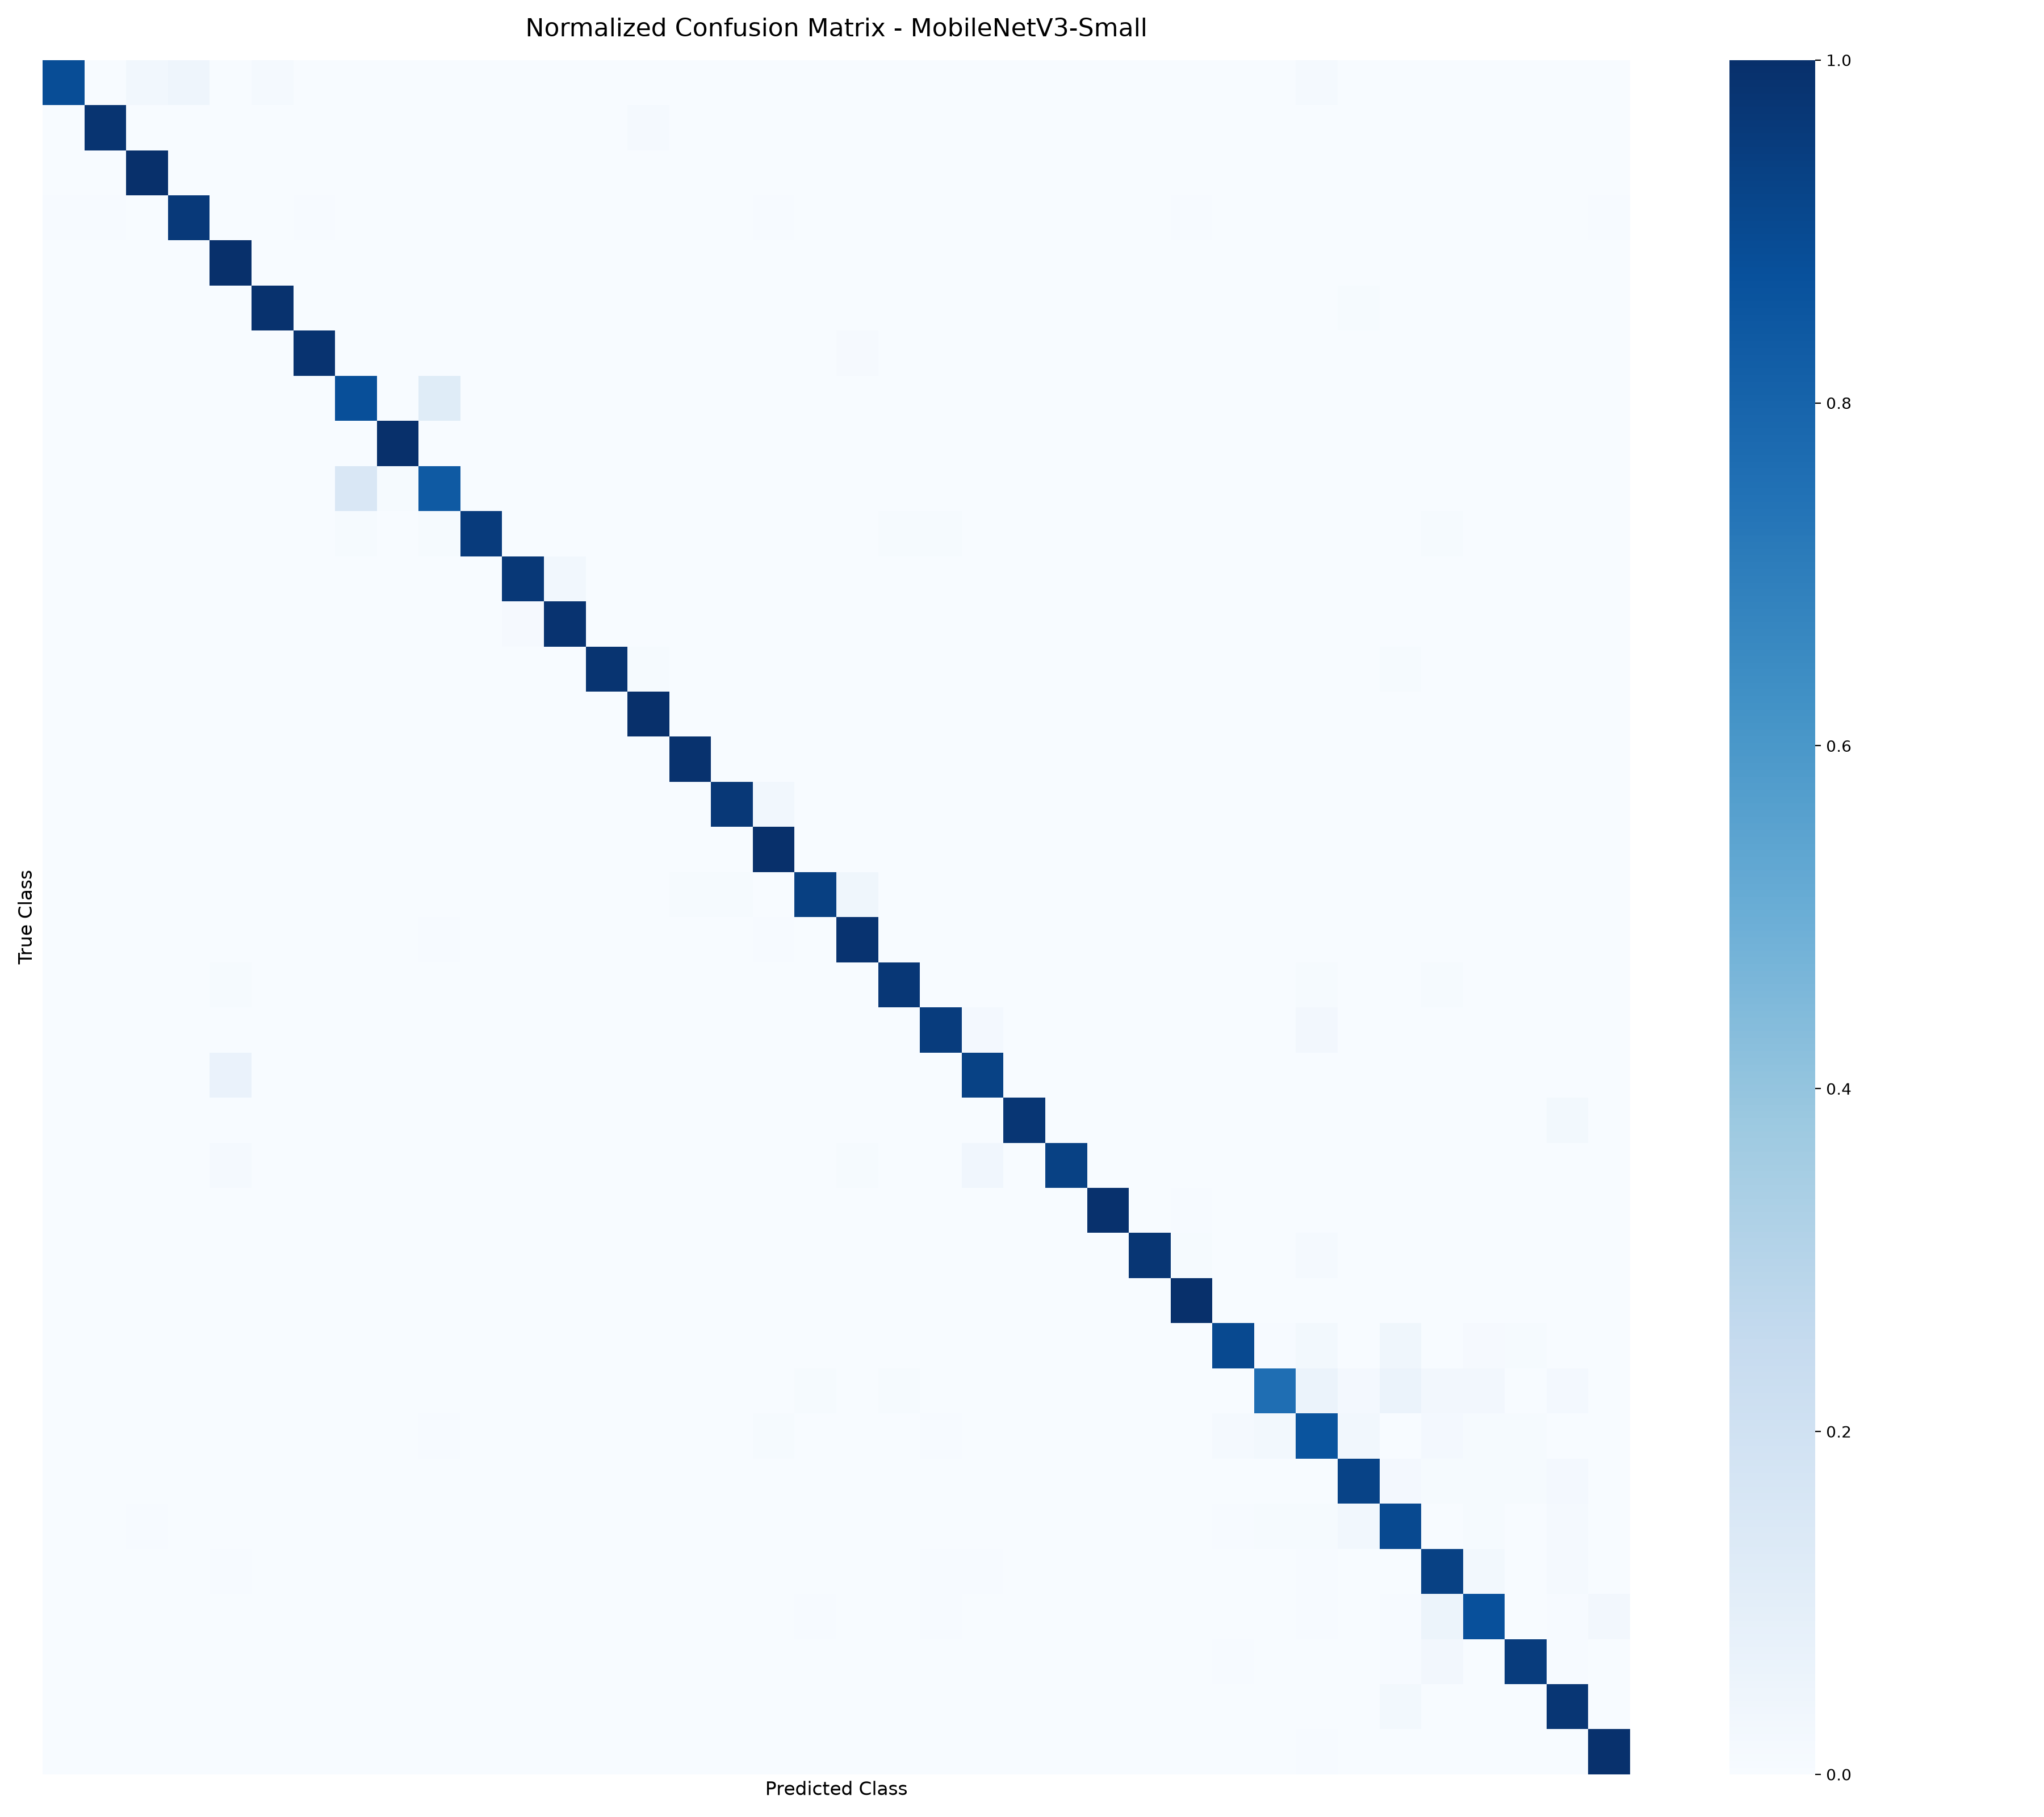
\includegraphics[width=0.48\textwidth]{figures/fig_confmat_mvs.png}\hfill
  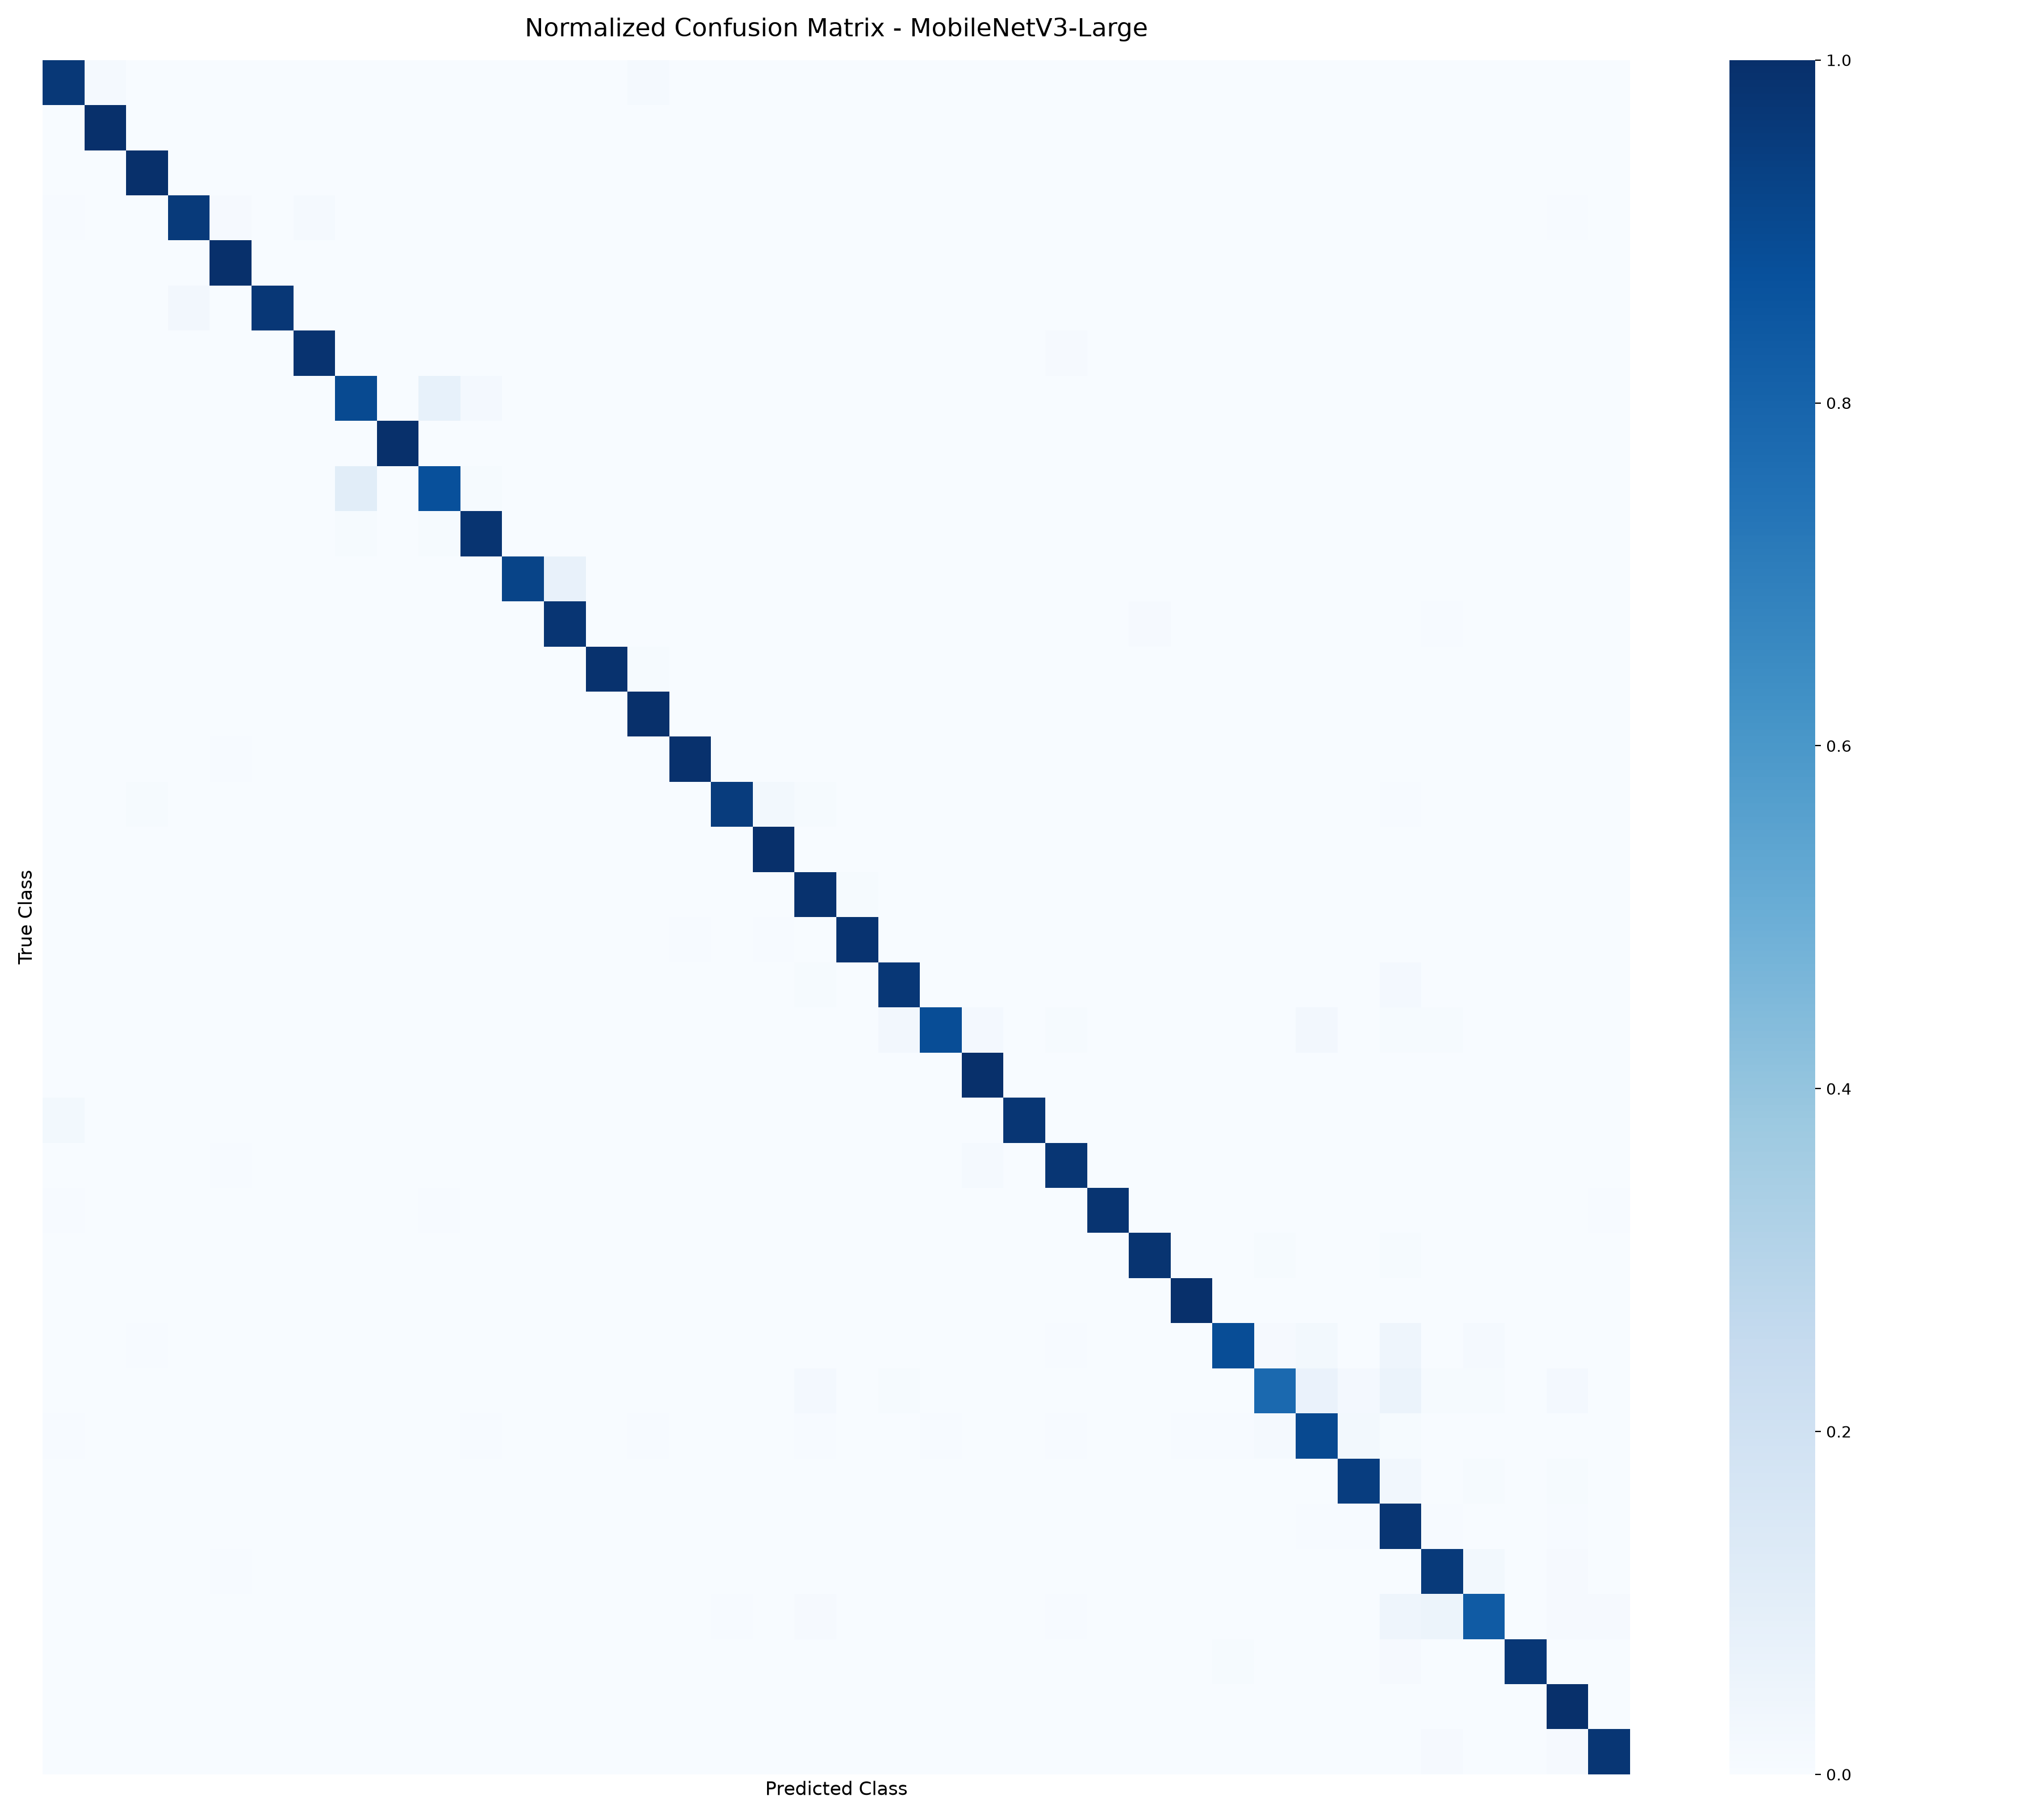
\includegraphics[width=0.48\textwidth]{figures/fig_confmat_mvl.png}
  \caption{Normalised 38-class confusion matrices on the PlantVillage holdout test partition (5{,}417 images). Left: MobileNetV3-Small; Right: MobileNetV3-Large. Rows represent true classes; columns represent predicted classes. Strong diagonal dominance is observed for both architectures. Off-diagonal errors are concentrated within the same host species.}\label{fig:confmat}
\end{figure}

\subsubsection{PlantDoc Domain-Shift Errors}

On PlantDoc, the calibrated ECE rises dramatically from 0.74\% (PlantVillage) to 21.86\%
(PlantDoc) for MobileNetV3-Small, confirming that the temperature parameters fitted on
controlled data do not transfer to unconstrained backgrounds. The NLL increases from
0.1637 to 2.5087, indicating a 15-fold degradation in probabilistic prediction quality.

\subsection{Comparative Architecture Analysis}
\label{sec:comparative_analysis}

Figure~\ref{fig:arch_comparison} provides a visual comparison of all four architectures
across accuracy, generalization, and efficiency metrics.

\begin{figure}[h]
  \centering
  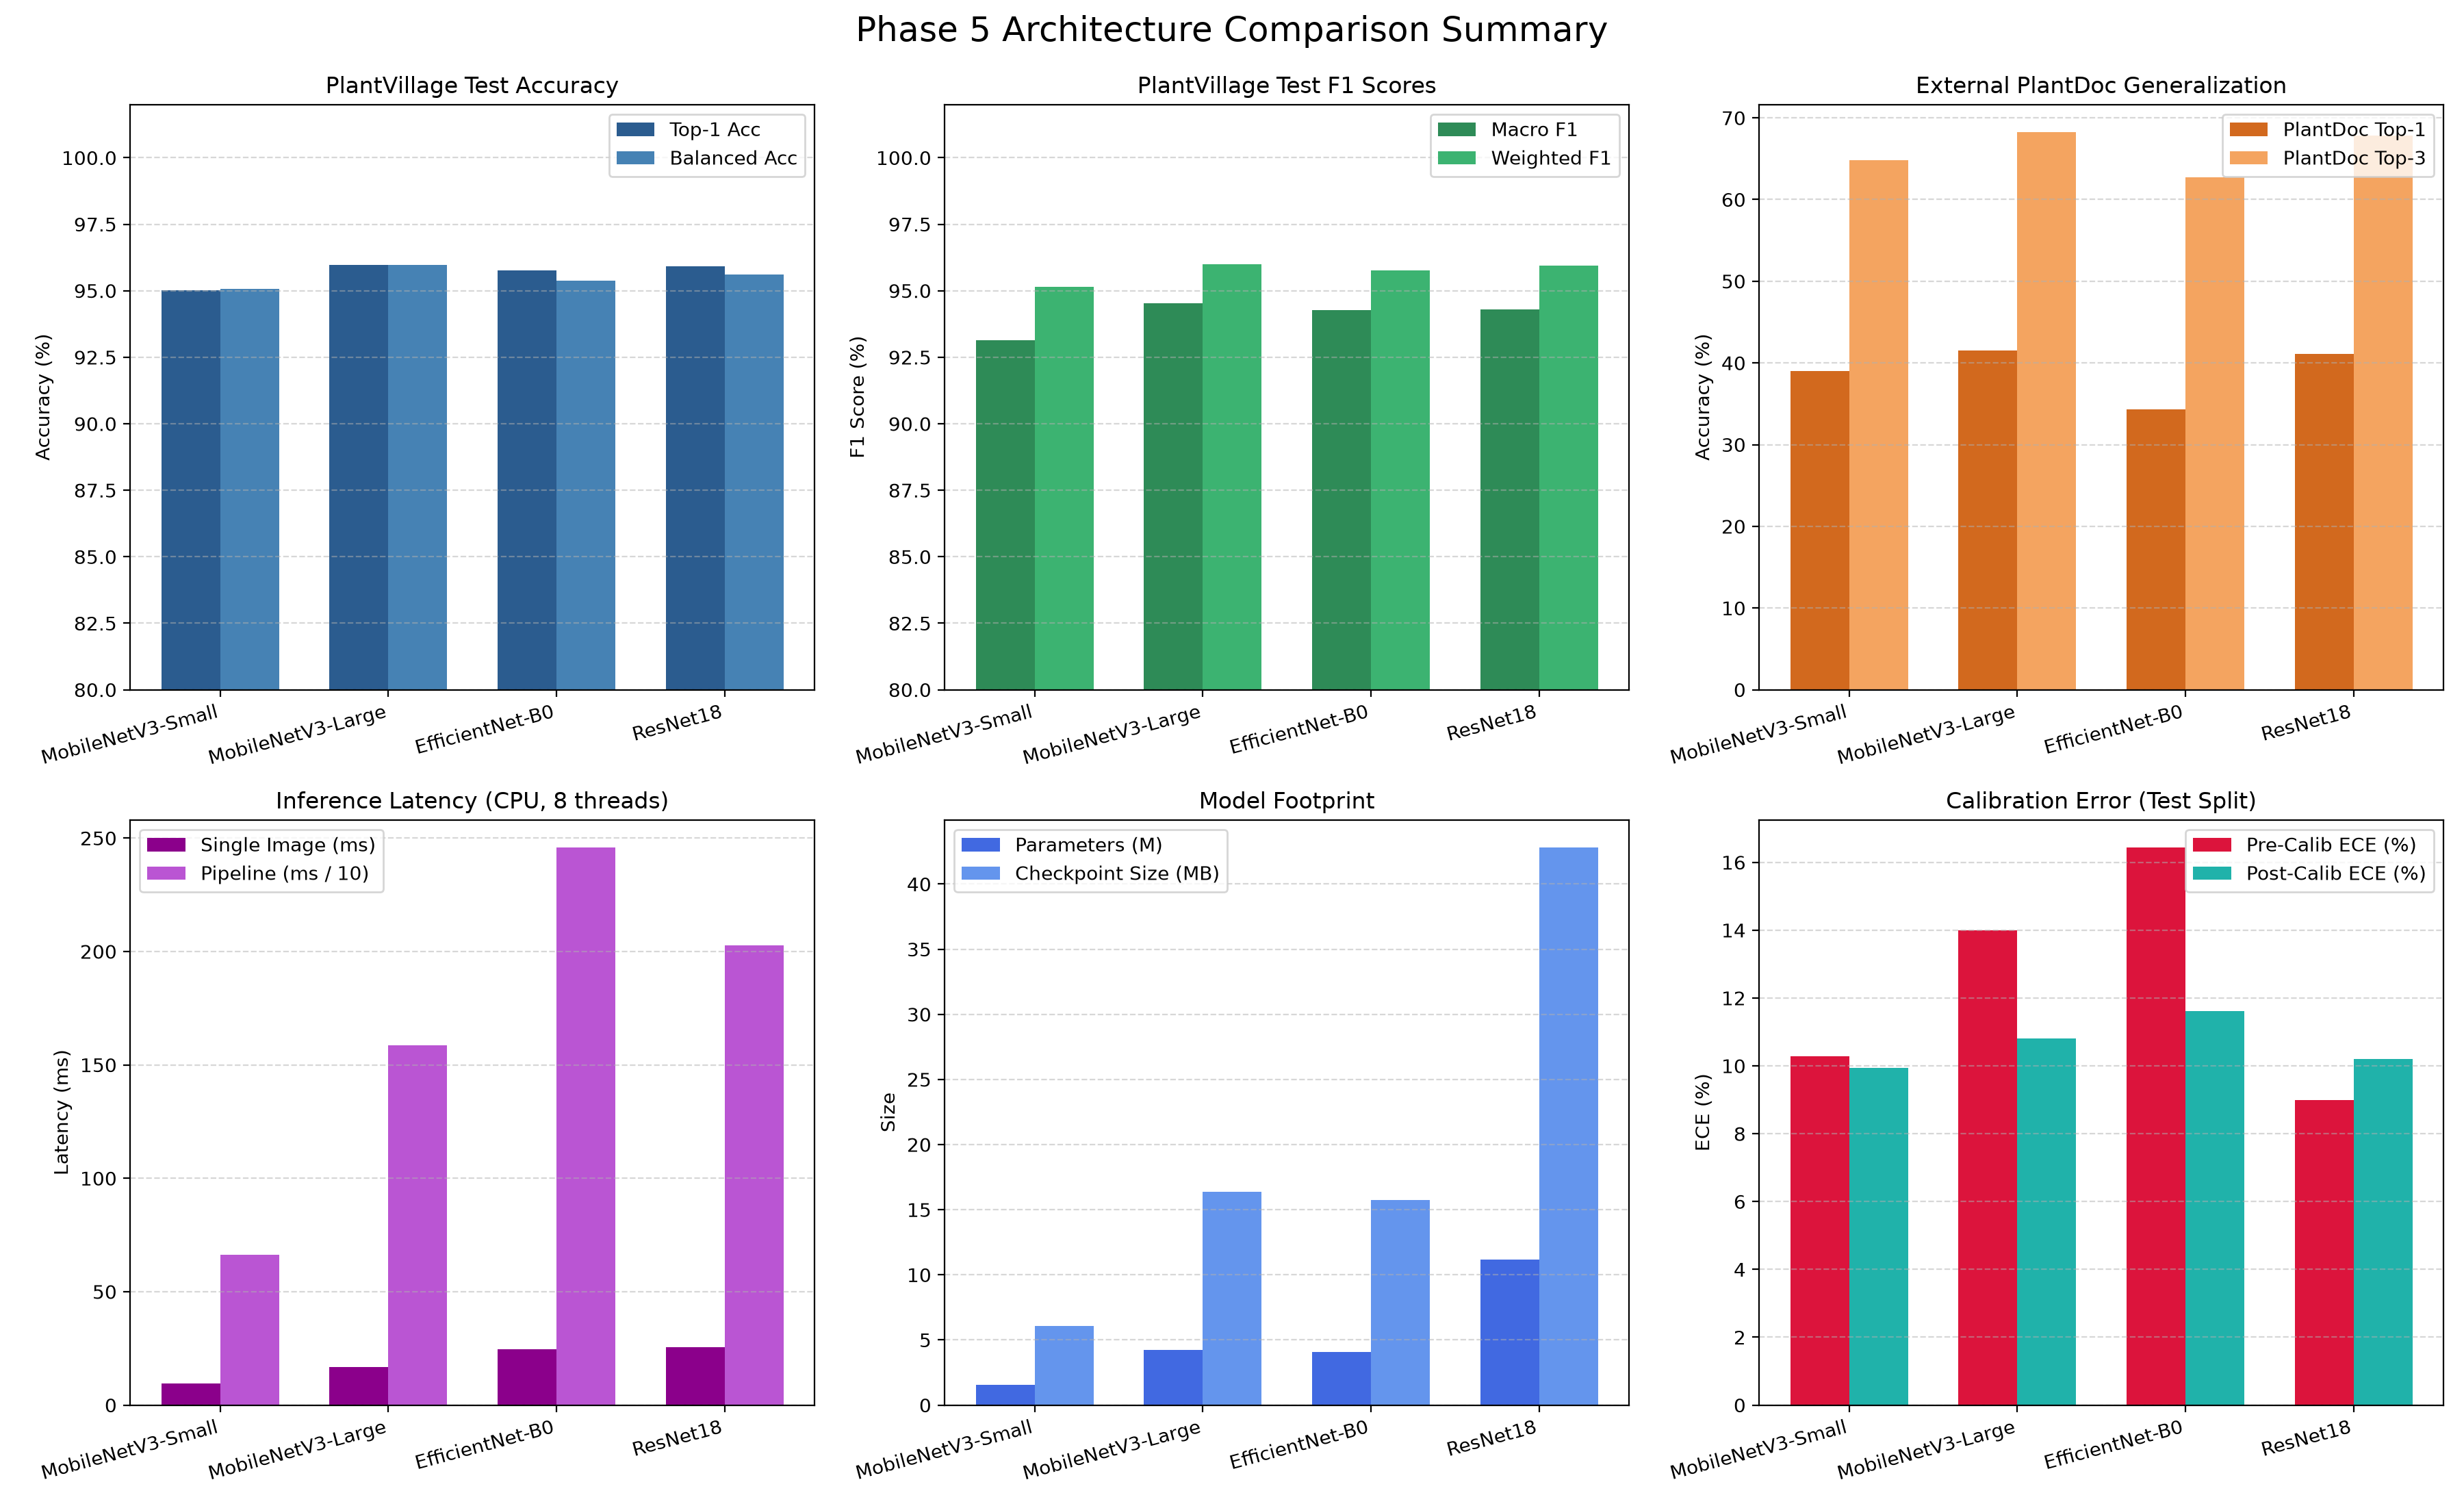
\includegraphics[width=\linewidth]{figures/fig_arch_comparison.png}
  \caption{Phase 5 architecture comparison across six evaluation dimensions:
  PlantVillage test accuracy, F1 scores, external PlantDoc generalization,
  CPU inference latency, model footprint, and calibration ECE. Each panel
  compares MobileNetV3-Small, MobileNetV3-Large, EfficientNet-B0, and ResNet18.}
  \label{fig:arch_comparison}
\end{figure}

Table~\ref{tab:full_comparison} consolidates the complete architecture comparison
including efficiency and screening pipeline metrics.

\begin{table}[h]
\caption{Comprehensive architecture benchmark: classification, generalization, calibration,
and efficiency. Single-image latency measured over 100 runs on AMD Ryzen 7 5800HS (8 CPU
threads). Pipeline latency includes ExG filtering, CNN inference, and hybrid NMS over
50 PlantDoc images.}\label{tab:full_comparison}%
\setlength{\tabcolsep}{3pt}%
\begin{tabular*}{\textwidth}{@{\extracolsep\fill}lrrrrrr}
\toprule
\textbf{Architecture} & \textbf{PV Acc} & \textbf{PV F1} & \textbf{PD Top-1} & \textbf{PD Top-3} & \textbf{Latency} & \textbf{Pipeline} \\
& \textbf{(\%)} & \textbf{(\%)} & \textbf{(\%)} & \textbf{(\%)} & \textbf{(ms)} & \textbf{(ms)} \\
\midrule
MobileNetV3-Small  & 95.02\% & 93.13\% & 38.98\% & 64.83\% & \textbf{9.42}  & \textbf{662} \\
MobileNetV3-Large  & \textbf{95.96\%} & \textbf{94.52\%} & \textbf{41.53\%} & \textbf{68.22\%} & 16.87 & 1{,}585 \\
EfficientNet-B0    & 95.77\% & 94.26\% & 34.32\% & 62.71\% & 24.58 & 2{,}457 \\
ResNet18           & 95.92\% & 94.30\% & 41.10\% & 67.80\% & 25.54 & 2{,}026 \\
\botrule
\end{tabular*}
\end{table}

\textit{Architecture selection guidance}: MobileNetV3-Small is optimal for
resource-constrained edge deployment where latency is critical. MobileNetV3-Large
offers the best balance of accuracy, generalization, and efficiency at moderate
parameter cost. EfficientNet-B0 and ResNet18 deliver competitive PlantVillage accuracy
but are slower and larger than the MobileNetV3 variants without commensurate
generalization benefits on PlantDoc.

\subsection{Candidate-Region Screening Evaluation}
\label{sec:results_screening}

Table~\ref{tab:screening_results} compares the Phase 4 baseline and Phase 4.1 optimized
screening pipeline on the 236-image PlantDoc official test benchmark (452 ground-truth
whole-leaf bounding boxes).

\begin{table}[h]
\caption{Candidate-region screening evaluation on the PlantDoc official test benchmark
(236 images, 452 whole-leaf bounding-box annotations). Ground-truth annotations
represent entire leaf boundaries, not lesion segmentation masks. Correctly classified
detections refers to candidate regions that (a) match a ground-truth leaf at
IoU $\geq 0.25$ and (b) are classified with the correct disease label.}\label{tab:screening_results}%
\setlength{\tabcolsep}{3.5pt}%
\begin{tabular*}{\textwidth}{@{\extracolsep\fill}p{4.2cm}rrp{2.2cm}}
\toprule
\textbf{Metric} & \textbf{Phase 4 Base} & \textbf{Phase 4.1 Opt} & \textbf{Change} \\
\midrule
Recall @ IoU 0.10        & 50.00\% & 62.17\% & +12.17 pp \\
Precision @ IoU 0.10     & 24.78\% & 17.31\% & $-7.47$ pp \\
Recall @ IoU 0.25        & 18.14\% & \textbf{38.05\%} & +109.8\% rel. \\
Precision @ IoU 0.25     &  8.99\% & 10.60\% & +17.9\% rel. \\
F1 @ IoU 0.25            & 12.02\% & \textbf{16.58\%} & +37.9\% rel. \\
Recall @ IoU 0.50        &  3.10\% &  7.96\% & +157\% rel. \\
Precision @ IoU 0.50     &  1.54\% &  2.22\% & +44.5\% rel. \\
Correct detections       & 30 leaves & \textbf{66 leaves} & +120.0\% \\
Crop accuracy            & 36.59\% & 38.37\% & +1.78 pp \\
FP per image @ IoU 0.25  &  3.52 &  6.15 & $+2.63$ \\
CPU latency (mean)       & 167.0\,ms & 844.2\,ms & +677.2\,ms \\
\botrule
\end{tabular*}
\end{table}

\begin{table}[h]
\caption{Stage-wise CPU latency breakdown of the candidate-region screening pipeline measured on an AMD Ryzen 7 5800HS processor (8 CPU threads). The un-attributed execution time in preliminary reports is verified as the candidate crop extraction, dynamic context padding, and tensor normalization stage.}\label{tab:latency_breakdown}%
\setlength{\tabcolsep}{4pt}%
\begin{tabular*}{\textwidth}{@{\extracolsep\fill}lrrp{4.0cm}}
\toprule
\textbf{Pipeline Stage} & \textbf{Baseline} & \textbf{Optimized} & \textbf{Execution Profile} \\
& \textbf{(ms)} & \textbf{(ms)} & \\
\midrule
Window Proposal Gen. (Multi-scale)       & 0.04 &   0.10 & \raggedright NumPy vectorized grid indexing \\
Foliar Saliency Pre-Filter (ExG)         & 0.00 &  24.16 & \raggedright NumPy array operations (CPU) \\
Crop Extraction \& Tensor Prep           & 67.07 & 358.19 & \raggedright PIL slicing, resize \& normalize \\
Batch Forward Inference (MobileNetV3-S)  & 99.87 & 461.62 & \raggedright PyTorch 2.15.0+cpu (8 threads) \\
Hybrid NMS \& Overlap Suppression        & 0.04 &   0.18 & \raggedright Pure Python greedy IoU loop \\
\midrule
\textbf{Total End-to-End Latency}        & \textbf{167.02} & \textbf{844.25} & \raggedright \textbf{Complete Screening Pipeline} \\
\botrule
\end{tabular*}
\end{table}

The Phase 4.1 optimised pipeline achieves substantial improvements in localization
recall at the practically relevant IoU threshold of 0.25, recovering 90 additional
ground-truth leaves (from 82 to 172 of 452) relative to the baseline. End-to-end
correct detections (localized and correctly classified) increased by 120\% from 30 to
66 leaves.

However, three important limitations must be acknowledged:
\begin{enumerate}
  \item \textbf{Precision remains low}: At IoU 0.25, precision is 10.60\%, implying
        that for every correctly localized leaf, approximately 8--9 spurious candidate
        windows are generated. These false positives originate primarily from background
        textures that pass the ExG filter but do not correspond to leaves.
  \item \textbf{Latency increase}: The optimised pipeline is 5$\times$ slower than
        the baseline (844 vs 167 ms/image), due to multi-scale candidate generation
        requiring more CNN forward passes. Sub-second latency is maintained but at
        higher CPU utilisation.
  \item \textbf{Dense canopy failure}: On images with $\geq 5$ leaves, recall drops
        to 21.88\% due to inter-leaf occlusion and aspect-ratio mismatch for elongated
        leaves such as maize and corn. Fixed-geometry sliding windows cannot resolve
        tightly overlapping canopy foliage without learned bounding-box regression.
\end{enumerate}

\textbf{Critical scope clarification}: The PlantDoc annotations describe whole-leaf
bounding boxes (mean box area: 30.08\% of image frame), not lesion segmentation masks
or necrotic-region annotations. Candidate regions produced by this pipeline are leaf
proposals, not disease localizations. Any claim of lesion-level segmentation or clinical
lesion area quantification would be unsupported by the available ground truth.

\subsection{Calibration and Computational Efficiency Summary}
\label{sec:efficiency_summary}

Figure~\ref{fig:calibration} illustrates the reliability diagrams for MobileNetV3-Small
under Phase 3 calibration ($T^* = 0.5538$), showing near-perfect alignment between
predicted confidence and empirical accuracy after scaling on the calibration partition.

\begin{figure}[h]
  \centering
  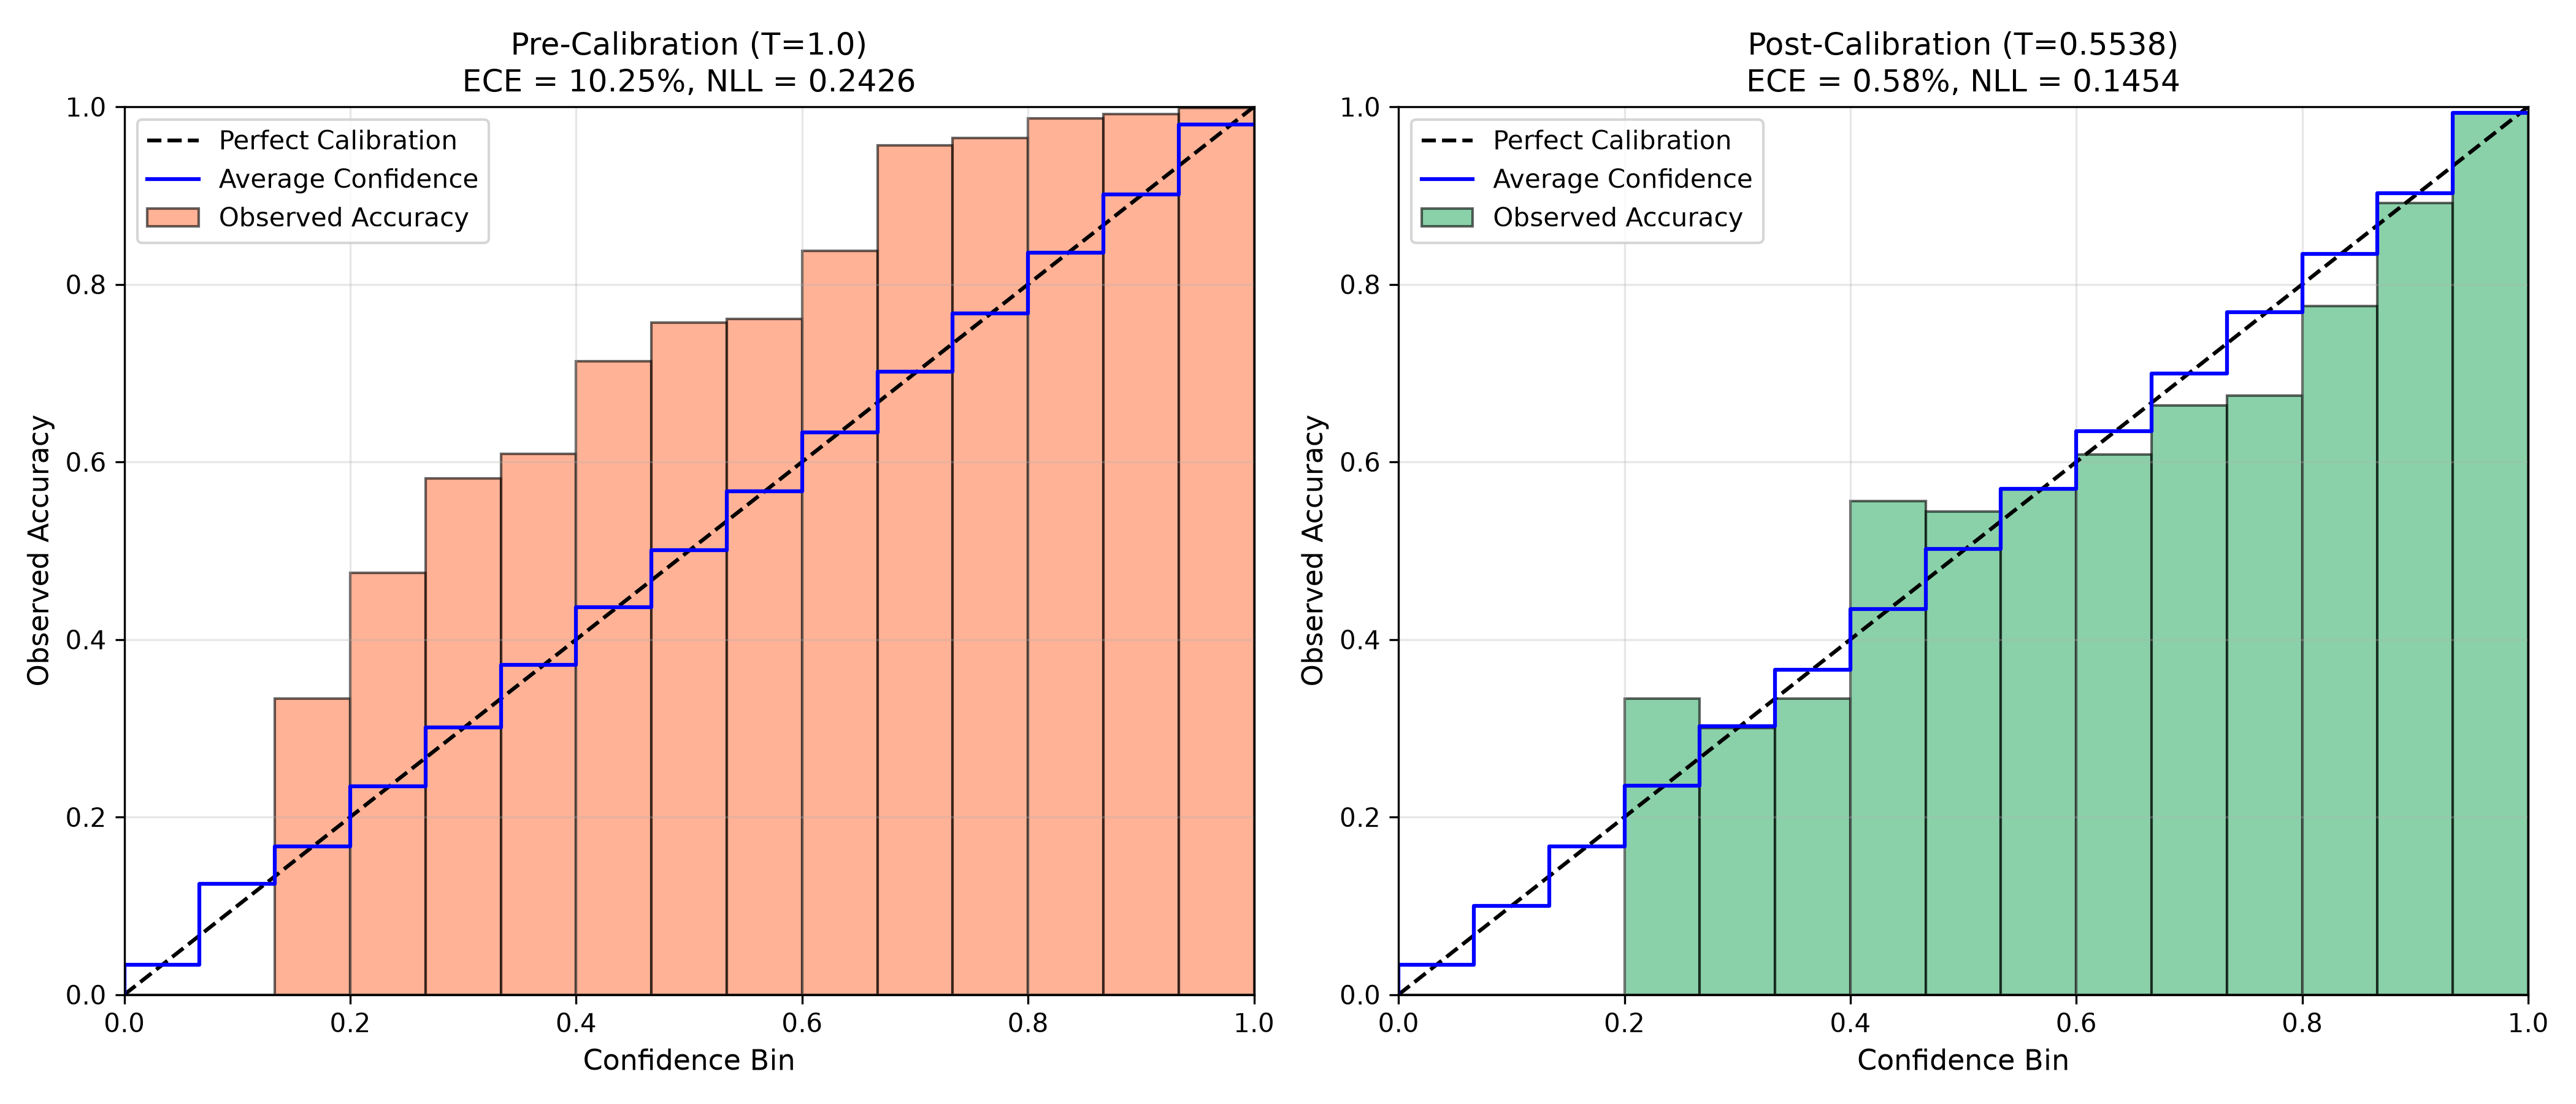
\includegraphics[width=0.9\linewidth]{figures/fig_calibration.png}
  \caption{Reliability diagrams for MobileNetV3-Small. Left: pre-calibration ($T=1.0$,
  ECE=10.25\%). Right: post-calibration ($T^*=0.5538$, ECE=0.58\%) on the 5{,}429-image
  calibration partition. Temperature scaling effectively aligns predicted confidence with
  empirical accuracy. Source: Phase 3 calibration experiment.}
  \label{fig:calibration}
\end{figure}

A three-tier confidence-based review policy was established using the calibration
partition, without accessing the test partition:
\begin{itemize}
  \item \textbf{Tier 1 --- Autonomous Acceptance} ($\tau \geq 0.70$): Coverage 94.5\%,
        accuracy 97.6\% on calibration data.
  \item \textbf{Tier 2 --- Secondary Human Review} ($0.40 \leq \tau < 0.70$):
        Flagged for agronomist inspection.
  \item \textbf{Tier 3 --- Mandatory Diagnostic Referral} ($\tau < 0.40$):
        Deferred to plant pathology clinic.
\end{itemize}

%% ================================================================
%% 5. CONCLUSION AND FUTURE SCOPE
%% ================================================================

\section{Conclusion and Future Scope}
\label{sec:conclusion}

This paper presents a comprehensive empirical evaluation of a CPU-deployable plant
disease screening system across five experimental phases, covering dataset construction,
architecture training, temperature calibration, candidate-region screening, and
multi-architecture comparative benchmarking.

\textbf{Key findings are summarised as follows}:
\begin{enumerate}
  \item All four architectures achieve competitive in-domain classification accuracy
        (95.02\%--95.96\%) on the controlled PlantVillage holdout test set, with
        performance differences within approximately one percentage point.
  \item MobileNetV3-Large achieves the highest holdout accuracy (95.96\%, Macro-F1
        94.52\%) and the strongest external PlantDoc generalization (41.53\% top-1).
  \item MobileNetV3-Small provides the best computational profile: 9.42\,ms inference
        latency, 6.06\,MB disk footprint, and 1.56M parameters, making it the preferred
        choice for resource-constrained edge deployment.
  \item The domain shift from controlled PlantVillage to natural PlantDoc conditions is
        severe ($\approx$56 percentage points) and consistent across all four architectures,
        confirming that in-domain benchmark accuracy does not predict field utility.
  \item Post-hoc temperature scaling is effective but its calibration gains are
        dataset-specific and do not transfer to PlantDoc natural-background conditions.
  \item The candidate-region screening pipeline more than doubles localization recall at
        IoU 0.25 (from 18.14\% to 38.05\%) through multi-scale windows, aspect-ratio
        awareness, ExG saliency filtering, context padding, and hybrid NMS, while
        increasing end-to-end latency to 844 ms per image.
  \item Precision at IoU 0.25 remains low (10.60\%), dense canopy recall is poor
        (21.88\%), and the pipeline is restricted to whole-leaf proposal generation and
        cannot perform lesion-level segmentation.
\end{enumerate}

\textbf{Future scope} to address the identified limitations includes:
\begin{enumerate}
  \item Domain adaptation and mixed-dataset fine-tuning using natural-background images
        to reduce the domain shift to PlantDoc and genuine field photographs.
  \item Integration of a learned leaf detection model (e.g.\ YOLOv8 or RT-DETR) trained
        on PlantDoc bounding-box annotations to replace heuristic sliding-window generation
        and improve precision-recall trade-offs.
  \item Pixel-level disease lesion annotation and semantic segmentation to enable
        clinically meaningful severity estimation.
  \item Open-set rejection mechanisms (e.g.\ energy-based or entropy-based out-of-distribution
        detection) to prevent erroneous confident classification of non-plant images.
  \item Prospective field validation through partnerships with agricultural extension
        services, covering diverse geographies, crop varieties, and growth stages.
  \item Full frontend application integration and user-facing deployment validation, which
        was deferred from the current experimental programme.
\end{enumerate}

The reproducible experimental infrastructure, verified checkpoints, and transparent
documentation of limitations established in this work provide a rigorous baseline for
future research in field-deployable plant disease AI.

%% ================================================================
%% CHECKPOINT PROVENANCE
%% ================================================================

\section*{Checkpoint Provenance and Reproducibility}

All trained model checkpoints are cryptographically verified. The combined split
manifest (SHA-256: \texttt{f9ef8b9d...15868}) ensures bit-for-bit data reproducibility.
Checkpoint SHA-256 digests are listed in Table~\ref{tab:checkpoints}.

\begin{table}[h]
\caption{Cryptographic checkpoint provenance for all Phase 5 benchmark models.
SHA-256 digests verify checkpoint integrity. Checkpoint paths are relative to the
project root \texttt{saved\_models/experiments/architecture\_benchmark/}.}\label{tab:checkpoints}%
\setlength{\tabcolsep}{3.5pt}%
\begin{tabular*}{\textwidth}{@{\extracolsep\fill}lrrl}
\toprule
\textbf{Architecture} & \textbf{Params} & \textbf{Size (MB)} & \textbf{SHA-256 (first 32 hex)} \\
\midrule
MobileNetV3-Small  & 1{,}556{,}806 &  6.06 & \texttt{6190f54c56ebbb7f4a663b5eb88a53c6} \\
MobileNetV3-Large  & 4{,}250{,}710 & 16.40 & \texttt{8ebfb512a071915ca9a7b508e52a9f3a} \\
EfficientNet-B0    & 4{,}056{,}226 & 15.74 & \texttt{faba42992b190b4c6c37409634070f0a} \\
ResNet18           & 11{,}196{,}006 & 42.79 & \texttt{f2991bef8630f6e162923fe3224d8d68} \\
\botrule
\end{tabular*}
\end{table}

\noindent Training was executed on Windows 10 Home (64-bit), AMD Ryzen 7 5800HS (8 physical cores, 16 threads, 3.20\,GHz), 16\,GB DDR4 RAM, Python 3.12.5, PyTorch 2.15.0+cpu, torchvision 0.29.2+cpu, OpenCV 5.0.0, NumPy 2.5.4, and Pillow 13.0.0. All experiments enforced \texttt{torch.use\_deterministic\_algorithms(True)} with seed 42.

\subsection*{Deterministic Reproduction Protocol}
The complete Phase 1--5 experimental pipeline is executed under deterministic controls via the following sequential command sequences:
\begin{enumerate}
  \item \textbf{Dataset Partitioning \& Combined Manifest Generation}:\\
        \texttt{python training/prepare\_splits.py --dataset-dir data/processed/PlantVillage --seed 42 --output-manifest reports/generated/combined\_split\_manifest.json}\\
        \textit{Verification Check:} Generates combined split manifest SHA-256 \texttt{f9ef8b9dcd6823f2021a0f24b94e2330adef4a7be01dc7bf1c652c0d6be15868} (56{,}433 records: 40{,}151 train, 5{,}436 val, 5{,}429 calib, 5{,}417 test).
  \item \textbf{Definitive MobileNetV3-Small Fine-Tuning}:\\
        \texttt{python training/train\_definitive.py --config training/config\_final.yaml}\\
        \textit{Operational Configuration:} 3 completed epochs, batch size 8, head warmup 1 epoch, initial lr 0.001, backbone fine-tune lr $10^{-5}$, label smoothing 0.10, seed 42. Checkpoint SHA-256 \texttt{6190f54c56ebbb7f4a663b5eb88a53c6f70926e482e084d76d624c2a12725009}.
  \item \textbf{Comparative Multi-Architecture Benchmarking}:\\
        \texttt{python training/train\_benchmark\_architecture.py --arch [mobilenet\_v3\_large|efficientnet\_b0|resnet18] --config training/config\_final.yaml}
  \item \textbf{Post-Hoc Probability Calibration}:\\
        \texttt{python training/evaluate\_classifier.py --config training/config\_final.yaml}\\
        \textit{Verification Check:} Fits optimal scalar $T^* = 0.5538$ via L-BFGS on 5{,}429 calibration samples, reducing calibration ECE from 10.25\% to 0.58\% (holdout test ECE from 10.28\% to 0.74\%).
  \item \textbf{Independent PlantDoc External Evaluation}:\\
        \texttt{python training/evaluate\_plantdoc.py --config training/config\_final.yaml}\\
        \textit{Verification Check:} Evaluates 236 natural-background test images, confirming 38.98\% Top-1 accuracy, 36.84\% Macro-F1, and selective prediction (93.22\% coverage, 40.91\% selective accuracy at threshold 0.2231).
  \item \textbf{Phase 4.1 Candidate-Region Screening Optimization}:\\
        \texttt{python scratch/run\_phase4\_1\_final\_test\_evaluation.py}\\
        \textit{Verification Check:} Evaluates 236 images (452 ground-truth leaves), confirming Recall@0.25 = 38.05\%, Precision@0.25 = 10.60\%, F1 = 16.58\%, 6.15 FP/img, and 844.25\,ms mean end-to-end CPU latency.
\end{enumerate}

%% ================================================================
%% LIMITATIONS AND ETHICAL STATEMENT
%% ================================================================

\section*{Limitations and Ethical Considerations}

This system is a research prototype and is not validated for clinical or commercial
agricultural deployment. The following limitations must be observed by any practitioner
considering use of these results:
\begin{itemize}
  \item PlantDoc external evaluation (41.53\% top-1) does not constitute evidence of
        field-readiness. Field conditions introduce far greater variability than any
        benchmark dataset captures.
  \item Candidate-region proposals represent \textit{whole-leaf} detections, not
        lesion boundaries. Disease severity estimation, lesion area quantification,
        and segmentation-based diagnosis require pixel-level annotations not available
        in this study.
  \item Temperature calibration parameters are fitted on PlantVillage calibration data.
        They may not generalize to PlantDoc or other out-of-distribution inputs.
  \item Frontend application integration was not completed in this study.
        No claims of end-to-end deployed system validation are made.
\end{itemize}


\backmatter

\bmhead{Supplementary Information}
The complete split manifest, evaluation logs, and configuration files are available for verification.

\bmhead{Data Availability}
The combined split manifest is cryptographically verified with SHA-256 digest \texttt{f9ef8b9dcd6823f2021a0f24b94e2330adef4a7be01dc7bf1c652c0d6be15868} and available in the project repository.

\bmhead{Code Availability}
All Python scripts, evaluation pipelines, and frozen configurations are preserved for reproducible execution under deterministic PyTorch configuration.

\section*{Declarations}
The authors declare that they have no competing interests. No external funding was received for this study.

%% ================================================================
%% APPENDICES
%% ================================================================

\begin{appendices}

\section{Agronomic Pathology Reference and Diagnostic Triage Guide}
\label{sec:appendix_e}

\subsection{Three-Tier Non-Autonomous Screening Protocol for Extension Workers}
To translate model outputs into responsible field decision support without claiming autonomous clinical diagnostic authority, we formalize a structured three-tier screening triage protocol:

\begin{itemize}
  \item \textbf{Tier 1 --- High-Confidence Screening Candidate ($p_{\text{calibrated}} \ge 0.70$):} The detected leaf region demonstrates visual symptom patterns matching a supported pathology with high statistical confidence. The system outputs bounding box localization, class attribution heatmaps, and a non-prescriptive symptom summary. An agronomic advisory note explicitly instructs the extension worker to verify foliar margins and local environmental preconditions before recommending cultural sanitation.
  \item \textbf{Tier 2 --- Low-Confidence Referral ($0.223 \le p_{\text{calibrated}} < 0.70$):} The localized region exhibits abnormal foliar coloration or early necrotic lesions, but the posterior probability falls below confident discrimination thresholds. The system outputs the top-3 differential diagnoses with calibrated likelihoods, flags the sample for manual inspection, and prevents any autonomous decision from being logged.
  \item \textbf{Tier 3 --- Inconclusive or Unsupported Scene ($p_{\text{calibrated}} < 0.223$ or ExG Coverage $< 8\%$):} The input image contains severe motion blur, off-target foliage, complex overlapping canopies, or unsupported plant species. The screening engine suppresses candidate proposals and advises the user to recapture the photograph under diffuse natural lighting with a single isolated leaf in view. Under no condition does Tier 3 report a disease label.
\end{itemize}

\begin{table}[h]
\caption{Agronomic differential triage matrix mapping foliar signs to operational escalation tiers across major crop categories. All prescriptive pesticide directives and quarantine mandates have been removed; actions are strictly restricted to non-autonomous human-in-the-loop inspection and extension clinic referral.}\label{tab:field_matrix}%
\setlength{\tabcolsep}{2.5pt}%
\begin{tabular*}{\textwidth}{@{\extracolsep\fill}p{2.3cm}p{3.2cm}p{2.5cm}p{3.6cm}}
\toprule
\textbf{Crop \& Target} & \textbf{Pathological Indicators} & \textbf{Abiotic Lookalikes} & \textbf{Screening Triage Protocol} \\
\midrule
Apple Scab (\textit{Venturia inaequalis}) & \raggedright Olive-green to velvety dark brown lesions on adaxial surface & \raggedright Sooty mold, spray residue, mechanical abrasive wind injury & \raggedright Tier 1: Foliar margin inspection; hand lens check; refer if $>15\%$ canopy affected. \\
Corn Leaf Blight (\textit{Exserohilum turcicum}) & \raggedright Elongated elliptical grayish-green or tan necrotic streaks & \raggedright Drought leaf scorch, nitrogen deficiency chlorosis, Stewart's wilt & \raggedright Tier 1: Scout lower canopy for lesion progression along veins; collect foliar press. \\
Grape Black Rot (\textit{Guignardia bidwellii}) & \raggedright Small circular reddish-brown spots with dark borders \& pycnidia & \raggedright Anthracnose, pesticide phytotoxicity, hail puncturing & \raggedright Tier 1: Cross-check petioles and fruit clusters for pycnidia; record GPS plot coordinates. \\
Potato Early Blight (\textit{Alternaria solani}) & \raggedright Concentric target-board rings with localized chlorotic halo & \raggedright Magnesium deficiency, physiological senescence, ozone flecking & \raggedright Tier 1: Differentiate concentric zonation; recommend physical soil and tissue testing. \\
Potato Late Blight (\textit{Phytophthora infestans}) & \raggedright Water-soaked irregular pale green lesions expanding to dark brown & \raggedright Frost injury, wind desiccation, bacterial soft rot & \raggedright Tier 1 (Urgent): Visual inspection for white sporulation; flag for priority diagnostic assay. \\
Tomato TYLCV & \raggedright Upward leaf curling, marginal chlorosis, stunted leaflets & \raggedright Aphid infestation, mechanical mite damage, physiological roll & \raggedright Tier 1: Scout underside of leaflets for whitefly vectors; refer to plant virology facility. \\
Low Confidence / Ambiguous & \raggedright Diffused chlorosis, atypical lesion shape, overlapping foliage & \raggedright Nutrient deficiencies (Fe, Zn), herbicide drift, senescence & \raggedright Tier 2: Defer automated classification; withhold diagnosis; refer image and leaf press. \\
Unsegmented / Extreme Occlusion & \raggedright Total leaf coverage $< 8\%$ of view, extreme motion blur, shadow & \raggedright Bark, soil, non-target background weeds, artificial mulch & \raggedright Tier 3: Suppress candidate inference; prompt user to rephotograph with neutral backing. \\
\botrule
\end{tabular*}
\end{table}

\subsection{Field Deployment Protocol and Mobile Image Capture Guidelines}
To minimize out-of-distribution false positives in practical operational settings, field agricultural extension officers must adhere to standardized image acquisition constraints before submitting candidates to the screening pipeline:
\begin{enumerate}
  \item \textbf{Foliar Isolation and Background Control:} Position the target leaf flat without folding or extreme curl. Where dense background weed cover or bare soil creates color interference, place a matte neutral surface (or shaded hand) directly behind the specimen. The leaf blade must occupy at least 35\% of the central viewfinder.
  \item \textbf{Diffuse Ambient Illumination:} Avoid capturing leaves under direct, harsh perpendicular sunlight, which produces specular reflection hotspots that saturate green-channel values and mimic viral chlorosis. Early morning diffuse light, overcast conditions, or manual body shading are required.
  \item \textbf{Lens Sanitation and Focusing:} Clean mobile camera lenses to prevent grease smearing that creates false halo artifacts. Maintain a distance of 15--25\,cm to ensure fine lesion micro-structures (e.g., fungal pycnidia, concentric rings) remain sharp and resolvable above the $224 \times 224$ input resolution threshold.
  \item \textbf{Multi-Angle Verification:} For suspected quarantine-grade pathogens (such as \textit{Phytophthora infestans}), capture at least two complementary views (adaxial top surface and abaxial underside) to confirm characteristic sporulation patterns prior to escalating mitigation measures.
\end{enumerate}

\end{appendices}

%% ================================================================
%% REFERENCES
%% ================================================================

\bibliography{references}

\end{document}

